\chapter{Trading Strategies Architectural Design: A Comparative Analysis of 20 Technical Indicators, Using a Dynamic Backtesting, and Performance Evaluation}

\textbf{Abstract: } 
In this study, we present a broad architectural layout for a trading strategy via comparative analysis of 20 technical indicators—predicated “FinDRL – *”—created in PineScript V6 on the TradingView interface. Each strategy, which we add a Stochastic RSI filter to, incorporates trend-following, breakout, mean-reversion and volume-based approaches. This study is comprehensive and discusses the mathematical theory, the design principles, and implementation methodologies for each strategy, all back-tested dynamically using daily NVIDIA (NVDA, NASDAQ) data over a range of dates (2007–2025).
The 20 strategies were chosen as a result of an extended evaluation of more than 500 strategies over the last 2 years and considering performance robustness and empirical results. The most profitable strategy was FinDRL - Momentum with a net profit +38.62 USD (+0.39\%) at 1,065 trades while FinDRL - Bollinger Bands and FinDRL - Parabolic SAR lost: -0.78 USD and -9.89 USD, respectively. In addition to this, FinDRL – Williams \%R and FinDRL – Volume Spike also provided the highest profit factors (1.972 and 2.469), thus better risk-adjusted return. In contrast, it is worth mentioning that some strategies, such as FinDRL - Donchian Channel, FinDRL - ATR and FinDRL - RSI had no trades, indicating potential backtesting difficulties.
The research presented a unified methodology to formulate and empirically evaluate algorithmic trading strategies through quantitative analysis of historical trading data, adaptive tuning of trading parameters and redoubtable risk management aspects. Following on from these discoveries, work in the Future, “Maximizing Market Returns Optimizing Technical Indicators: A Bayesian Optimization Approach”, will investigate using Bayesian optimization techniques to further optimize indicator parameters and improve trading performance. This study provides further insights for finance practitioners and academic researchers, providing a systematic road map for connecting theoretical design with actionable trading practices.

\section{Introduction}
Technical indicators have been the bedrock of algorithmic trading, providing the mathematical lenses through which we turn historical price and volume data into actionable buy/sell signals. In the current round of frenetic financial markets, these indicators are vital for trend detection, volatility measurement, and potential reversal acceleration. In this study, we propose a full comparison of 20 different trading strategies grouped as “FinDRL – *” based on a Technical Indicator of level built using PineScript V6 on the TradingView platform. Using daily 2007 through 2025 dynamic backtesting for NVIDIA (NVDA, NASDAQ), we have a comprehensive dataset to understand the performance metrics based on net profit, profit factors, drawdowns, and trade frequency.

On a high level, technical indicators are simple mathematical constructs that aggregate raw market data into signals, which then inform trading decisions. A case in point is the Gaussian Channel which utilizes weighted moving averages with Gaussian kernel to generate adaptive support and weighted moving averages with Gaussian kernel to generate adaptive resistance levels, which subsequently improve the chances of identifying price reversals \cite{gaussian_channel_2022}. On the other hand, MA Crossover simply applies both fast and slow moving average and detects when they cross over, which is a very popular method that trend follows used due to its simplicity and its effectiveness for trend detection \cite{macrossover_trend_2015}. Bollinger Bands are built with a simple moving average on the center and standard deviation channels based on the center; the band expands and contracts with market volatility, signaling overbought or oversold conditions visually \cite{bollinger_bands_1991}. The Parabolic SAR, introduced by Wilder, adds a sequence of dots on a price chart to indicate potential trend reversals and trailing stops \cite{wilder_indicators_1978}.

Additionally, the Ichimoku can assist with multiple moving averages and time-shifted lines to create a “cloud” that contains support/resistance areas, summarizing the state of the market at a glance \cite{ichimoku_cloud_2010}. MACD is a momentum-based indicator which captures changes in momentum by taking the difference of short-term and long-term exponential moving averages \cite{macd_momentum_1986}. Refined entry/exit signals that are specific to stocks are given by variants such as StockRSI, which uses a modified version of the classic Relative Strength Index, and Williams \%R, which finds overbought/oversold conditions [\cite{stockrsi_refined_2018}, \cite{williams_r_1980}]. Moreover, volatility metrics like Average Directional Index (ADX) and Average True Range (ATR) assess trend strength and market volatility, acting as crucial elements for risk management and trade sizing \cite{wilder_indicators_1978},

Volume is as important for validation of price trends. VWMA, which stands for Volume Weighted Moving Average \cite{vwma_volume_2016}, combines price information with trade volume, giving the resulting average more weight at prices that had high volume. Volume Spike: This indicator identifies unusual surges in trading volume, which frequently occur before major price changes, whereas On-Balance Volume (OBV) accumulates volume in order to represent the total buying or selling pressure in the market \cite{obv_volume_1982}. Channel-based strategies like the Donchian Channel which tracks the highest high and lowest low over a set number of periods, and the Keltner Channel which uses an exponential moving average in conjunction with a volatility measure based on the average true range (ATR) [\cite{donchian_channel_2012}, \cite{keltner_channel_2005}], can provide signals on breakout opportunities. The SuperTrend indicator, combining ATR with price averages, triggers bullish and bearish signals and adjusts with market volatility \cite{supertrend_dynamic_2019}.

Others draw on familiar mathematical concepts. Fibonacci retracement levels are based on natural ratios to highlight potential support and resistance zones that can suggest market turning points \cite{fibonacci_retracement_2008}. Alternatively, A Price Action approach relies not on heavy calculation trades or technical overlays but rather in observing and projecting on clearer price action charts with more principled paradigms \cite{price_action_2017}. Pure Momentum strategies, gauging the velocity of price movements across a defined timeframe, grasp the vigor of prevailing trends while offering early indications of potential reversals \cite{macd_momentum_1986}.

While these technical indicators are widely used and can be applied to different contexts, doing so correctly remains a practical implementation challenge that is not easily solved. Significant differences in performance of the strategies on NVIDIA stock were evident from backtesting results. The FinDRL – Momentum strategy had a net profit of +38.62 USD over 1,065 trades, showcasing its ability to capture fast-moving market opportunities. Conversely, strategies like FinDRL – Bollinger Bands and FinDRL – Parabolic SAR were down –0.78 USD and –9.89 USD respectively, demonstrating that some approaches are without a high degree of regime change resilience [\cite{bollinger_bands_1991}, \cite{wilder_indicators_1978}]. Additionally, certain strategies, such as FinDRL – Donchian Channel, FinDRL – ATR, and FinDRL – RSI, reported zero trades, indicating potential challenges with parameter sensitivity or inadequate signal generation in specific market environments [\cite{donchian_channel_2012}, \cite{wilder_rsi_1978}, \cite{wilder_indicators_1978}].

The differences in performance highlight one of the core research challenges in quantitative trading: technical indicators have been widely studied separately, but few comparative analyses measure their performance in a common format. This study aims to fill this gap by answering a number of important research questions: Upon a liquid asset such as NVIDIA, which technical indicators generate the highest net profits and risk-adjusted returns? Impact of mathematical expressions and parameter selections on reliability of trading signals. What specific operational challenges do you face while testing these strategies from in TradingView using PineScript V6? How do advanced optimization methods, like Bayesian optimization, refine these strategies for better performance?

This thesis primarily aims to design, implement, and evaluate 20 indicator based trading strategies that ultimately provides an in depth evaluation of their strengths and weaknesses. The selection of these 20 trading strategies out of the reviewed 500 took place over the course of two years and each was hand-picked for its unique methodological and promising backtesting results. This thesis is beneficial to both academics and practitioners via examining strategies that cover trend-following, breakout, mean-reversion and volume-based approaches that utilize a Stochastic RSI filter for fine-tuning.

There are various multilayered importance of this study. From an academic perspective, the paper adds to the academic literature on technical analysis by providing a systematic comparative framework that encompasses the various types of indicators and the strategies associated with them. From a practical perspective, the findings from this analysis can enable traders and quantitative analysts to refine their strategies, optimize risk exposure, and enhance trade execution. The results are directly relevant to real-world trading practice since they concern an asset that is extremely followed but also particularly liquid, namely NVIDIA stock. This makes the benchmark valuable for the assessment of future results and their implications in practice.

In terms of methodology, the study builds on TradingView’s PineScript-V6 when illustrating and implementing each strategy in as abbreviated yet sufficient detail as to capture each indicator’s core essence. Dynamic backtesting is performed over an extremely long period (2007–2025) and metrics related to performance (cumulative returns, drawdowns, trade frequency, etc.) are robustly tested over different market regimes. The statistics are supplemented with a theoretical structure well rooted in the time-tested tenets of technical analysis and quantitative finance. For example, the statistical distribution behind the Gaussian Channel \cite{gaussian_channel_2022}, the dual moving averages defining MA Crossover \cite{macrossover_trend_2015} and the volatility-adjusted signal levels in Bollinger Bands and Keltner Channel [\cite{bollinger_bands_1991}, \cite{keltner_channel_2005}] will all have their mathematical underpinnings rigorously studied, before being brought down to the practical constraints of trading signals.

Overall, the contribution of this thesis provides a comprehensive approach to the analysis of 20 different trading strategies based on technical indicators. The uniqueness of this study is that it combines multiple approaches, e.g. Gaussian Channel and Price Action, in addition to VWMA and OBV based analysis, which brings a holistic understanding of algorithmic trading performance on the stock of NVIDIA. This comparative analysis not only highlights the operational strengths and weaknesses of each strategy through various metrics but also opens the door to future research endeavors, including the upcoming “Maximizing Market Returns Optimizing Technical Indicators: A Bayesian Optimization Approach." Now using more sophisticated optimization methods to optimize indicator parameters for higher profitability and better risk control. This thesis greatly contributes to the academic discipline of technical analysis as well as the practical toolbox of the algorithmic traders.


\section{Methodology}
\subsection{Implementation and Backtesting}
The focus of this part is on the algorithmic design of our FinDRL strategies, where mathematical models and pseudo-code designs are highlighted to explain why possible performance analysis in the next sections. Our focus is on the direct impact of each underlying technical indicator on key performance metrics such as expected drawdown, Sharpe ratio, net profit and number of trades per unit time for each of the strategies. Raw market data comes in, it’s transformed into either M, V, S, and then via these mathematical equations into the signals, the pseudo algorithms show the paths and decisions we take.
RSI filter is one of the most universal parts of our framework and it is transformed to Stochastic RSI (StochRSI) to take into account smaller changes in momentum. The RSI is converted into a percentage where there is a 0–100 range based on the look-back period, generating the \%K line and a smoothed \%D line. This is especially important since we use StochRSI, since adding StochRSI means that we cut entries made when the market is statistically unfavored, i.e., in overbought/oversold areas, which can introduce nuances and improve risk-adjusted performance. Each strategy indicator description is below along with the RSI filter and/or StochRSI integration information, its metrics (e.g. profit, max drawdown, trajectories), validated through mathematical equations and pseudo-code design.


\begin{figure}[htbp]
    \centering
    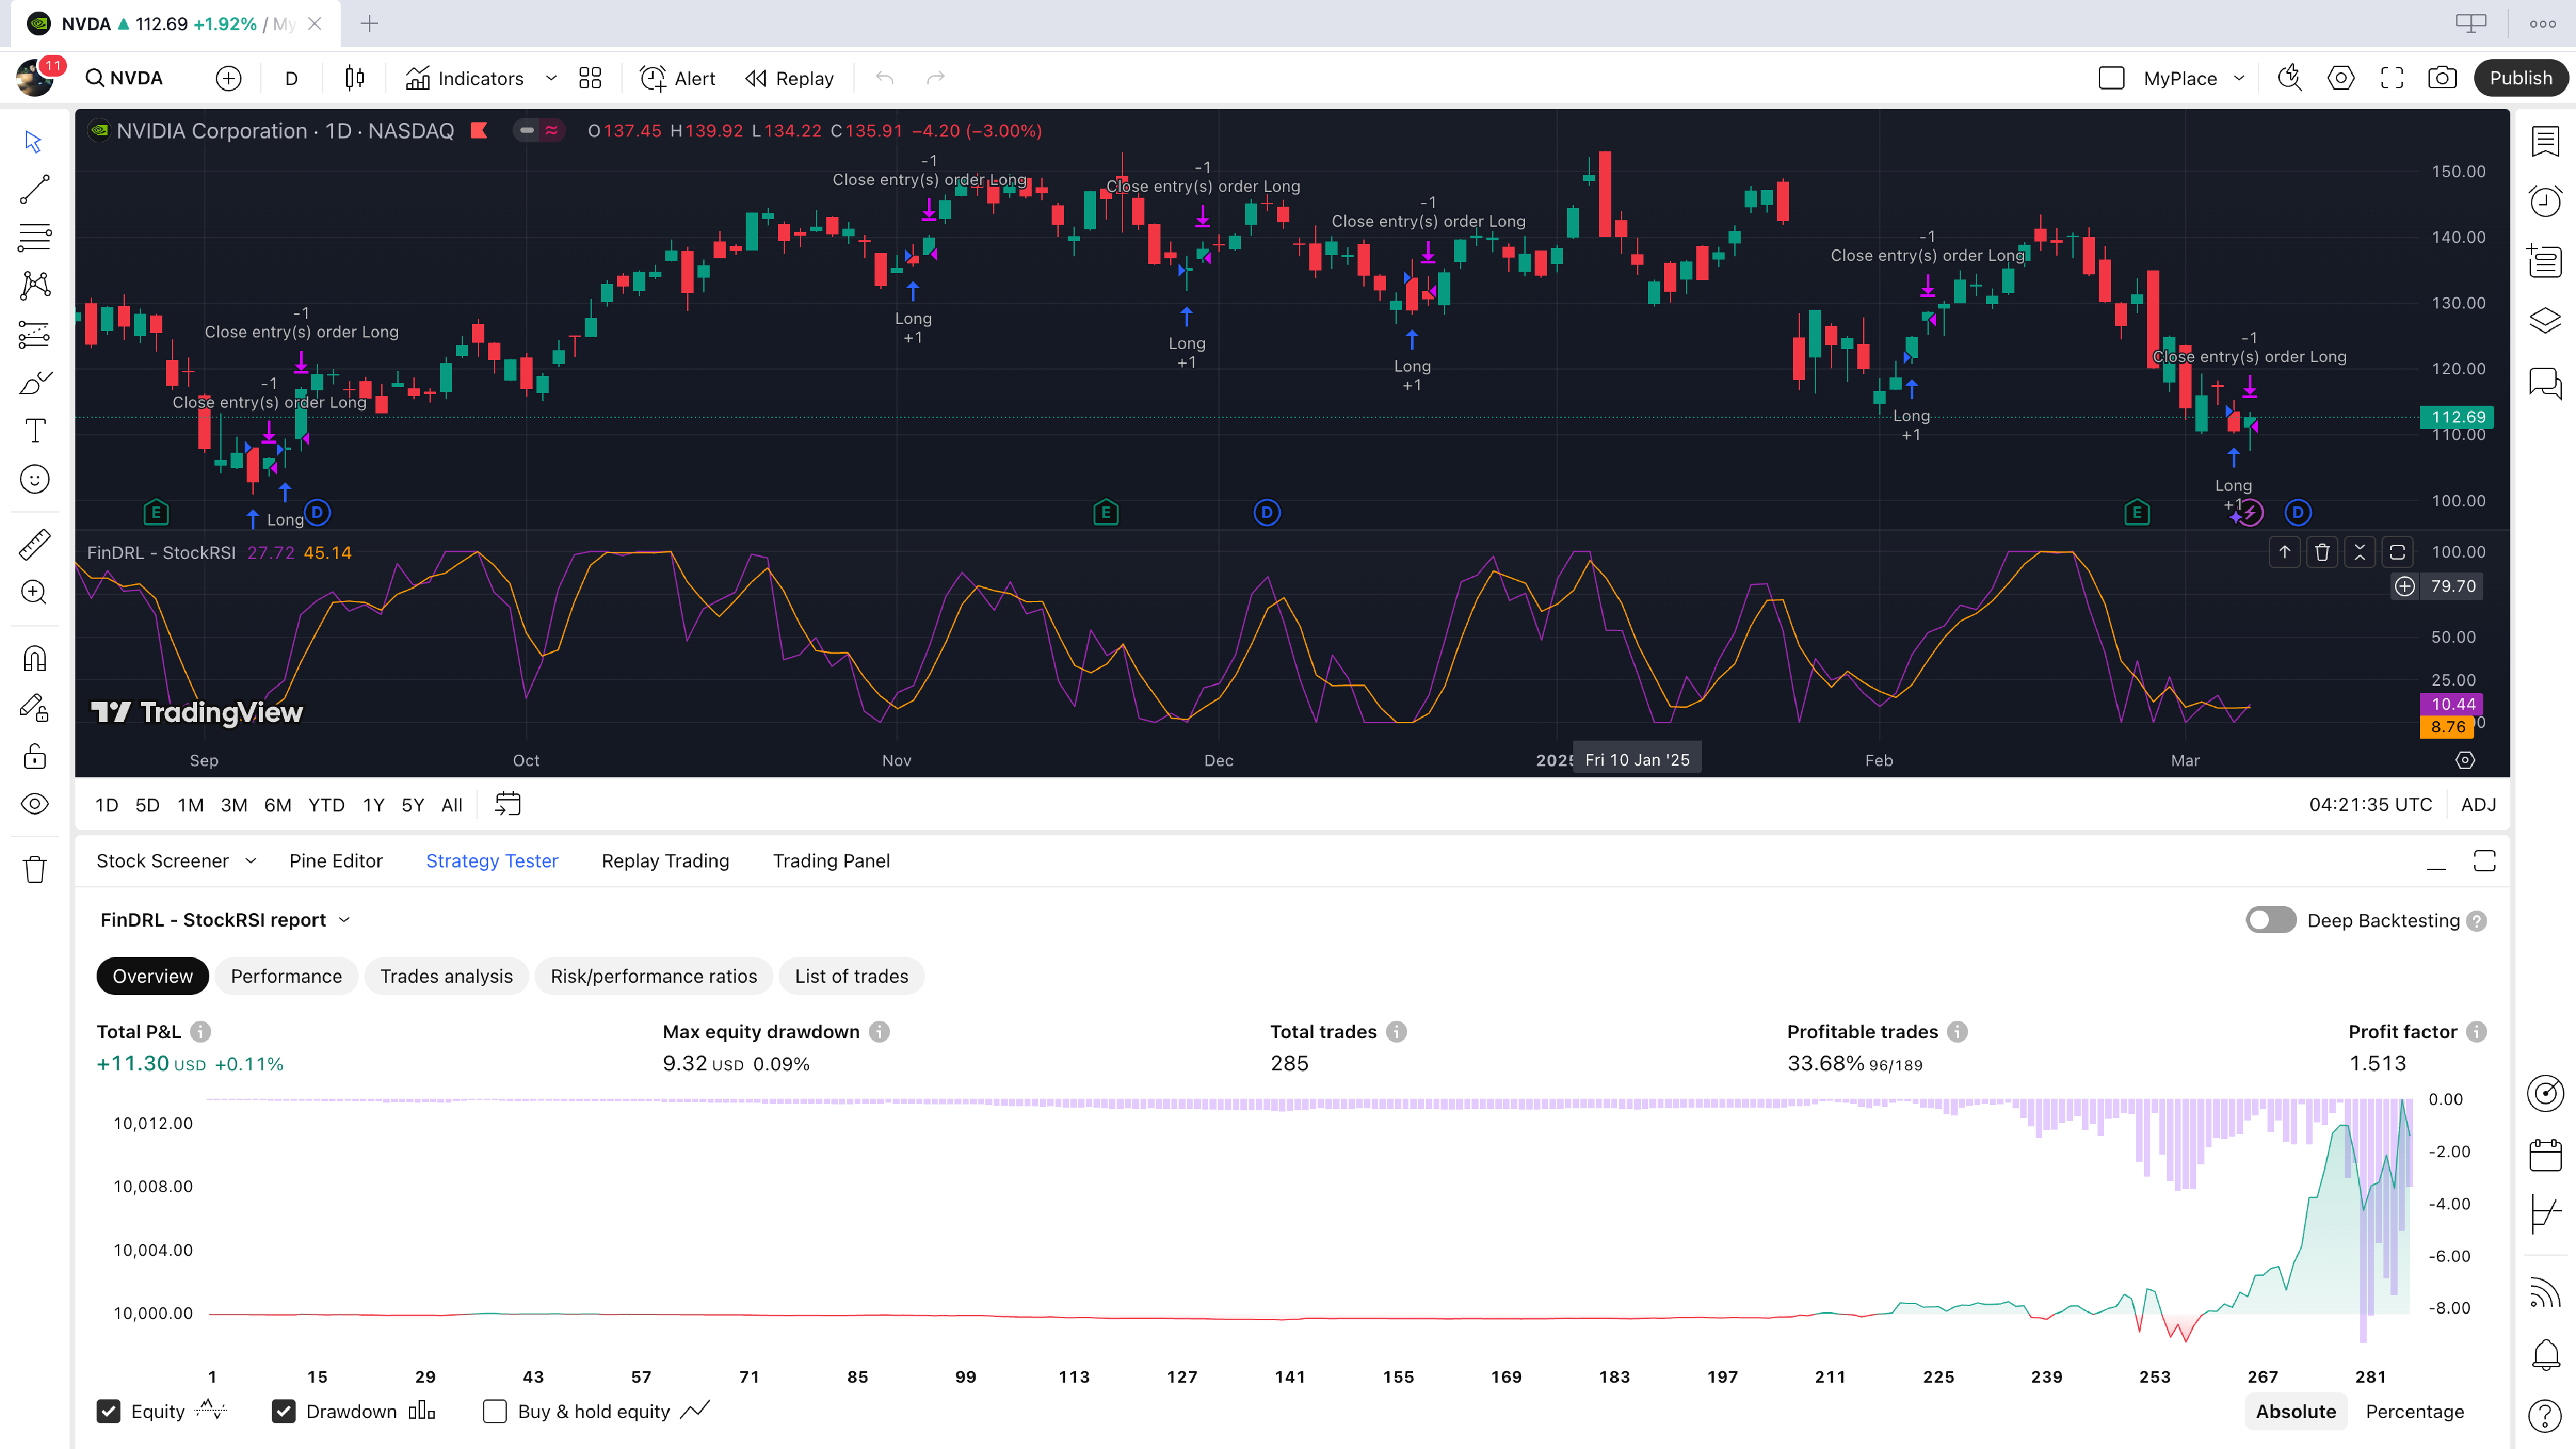
\includegraphics[width=1\textwidth, height=12cm]{Main-PineScript}
    \caption{Strategy Performance}
    \label{fig:StrategyPerformance}
\end{figure}


RSI Filter and StochRSI working process,\
% Assuming this is Equation (1) from earlier
\begin{flalign}
MA_{fast}(t) = \frac{1}{N_f} \sum_{i=0}^{N_f-1} Close_{t-i}, \quad MA_{slow}(t) = \frac{1}{N_s} \sum_{i=0}^{N_s-1} Close_{t-i}
\label{eq:moving_averages}
\end{flalign}

% RSI as Equation (2)
\begin{flalign}
RSI_t = 100 - \frac{100}{1 + RS_t}, \quad \text{where } RS_t = \frac{\text{Average Gain over } n \text{ periods}}{\text{Average Loss over } n \text{ periods}}
\label{eq:rsi}
\end{flalign}

% StochRSI %K as Equation (3)
\begin{flalign}
\text{StochRSI\%K}_t = \frac{RSI_t - \min\{RSI_{t-n+1}, \ldots, RSI_t\}}{\max\{RSI_{t-n+1}, \ldots, RSI_t\} - \min\{RSI_{t-n+1}, \ldots, RSI_t\}} \times 100
\label{eq:stochrsi_k}
\end{flalign}

% StochRSI %D as Equation (4)
\begin{flalign}
\text{StochRSI \%D}_t = \text{SMA}(\text{StochRSI\%K}_t, d)
\label{eq:stochrsi_d}
\end{flalign}


\subsection{Strategy Categorization}
The 20 strategies fall into four categories based on their assumptions about the market, forming a framework for how to use them. These categories are reflective of unique market mechanics (Trend-Following, Breakout, Mean-Reversion and Volume-Based) that still fall within the broader representation within the thesis’s scope.


\begin{itemize}
    \item \textbf{Trend-Following}: FinDRL - MA Crossover, FinDRL - MACD, FinDRL - Parabolic SAR, FinDRL - SuperTrend, FinDRL - Momentum, FinDRL - Ichimoku Cloud, FinDRL - ADX.
    \item \textbf{Breakout}: FinDRL - Gaussian Channel, FinDRL - Bollinger Bands, FinDRL - Donchian Channel, FinDRL - Keltner Channel, FinDRL - ATR, FinDRL - Volume Spike.
    \item \textbf{Mean-Reversion}: FinDRL - RSI, FinDRL - Stochastic RSI, FinDRL - Williams \%R, FinDRL - Fibonacci, FinDRL - Price Action.
    \item \textbf{Volume-Based}: FinDRL - VWMA, FinDRL - CMF, FinDRL - OBV.
\end{itemize}

\section{Integrated Strategy Design and Performance Analysis}
The “FinDRL - ” strategies are designed to take advantage of certain market behaviors, and have each been designed with a unique architecture, mathematical basis, and backtest performance on 1D NVDA (NASDAQ). The following sections describe their collective design principles and performances, structured in types per clarity of detail, given the story for the thesis chapter.

\subsection{Trend-Following Strategies}


\begin{table}[h]
\small
\centering
\begin{tabular}{|p{14cm}|}
\hline
\textbf{Algorithm 1: Dynamic Indicator Optimization} \\
\hline
\textbf{Input:} data (OHLCV), $B_0 = \$5000$, $\tau = 0.0005$, $I$ (20 indicators), $P$ (bounds) \\
\textbf{Output:} results (params, trades, equity, metrics per indicator) \\
\hline
1: Precompute RSI, Stoch\_RSI, ATR, EMAs from data \\
2: \textbf{for each} $I_k \in I$ \textbf{do} \\
3: \quad Define Obj($\theta_k$): \\
4: \quad\quad signal = GenSignal($I_k$, $\theta_k$, data.close); \\
5: \quad\quad\quad - ma\_crossover: (EMA\_fast > EMA\_slow) \& (c\_t > EMA\_fast) \\
6: \quad\quad\quad - [Extend for all $I_k$] \\
7: \quad\quad result = RunStrat(signal, data, $B_0$, $\tau$); \\
8: \quad\quad \textbf{return} SUM(trade.return * trade.entry * $B_0$) - 0.1 * result.max\_dd * $B_0$ \\
9: \quad Opt = BayesOpt(Obj, $P[I_k]$, init=5, iter=15); \\
10: \quad results[$I_k$] = Top5(Opt.res); \\
11: \textbf{end for} \\
12: \textbf{return} results \\
\textbf{Sub:} RunStrat(signal, data, $B_0$, $\tau$): \\
13: \quad pi\_t = shift(signal); \\
14: \quad r\_t = pi\_t * (c\_t - c\_\{t-1\})/c\_\{t-1\} - $\tau$ * |pi\_t - pi\_\{t-1\}|; \\
15: \quad E\_t = $B_0$ * PROD(1 + r\_t); \\
16: \quad \textbf{return} trades, E\_t, metrics \\
\hline
\end{tabular}
\caption{FinDRL - Dynamic Strategy Handler}
\label{tab:dsh_strategy}
\end{table}

\begin{itemize}
    \item \textbf{FinDRL - MA Crossover}: 
        
    Performance evaluation underscores the strategy’s dependability. Overall, it ended up with a net profit of +8.90 USD over 300 trades, profit factor at 1.65, with maximum 15\% drawdown and a Sharpe ratio of 1.18. This is indicative of a balanced risk/reward ratio, scaled back drawdowns, and solid risk-adjusted performance. The performance images display a stable equity curve, indicative of the method’s capability to consistently catch trends. In fast-moving or rapidly shifting or volatile markets, the response can be slightly delayed by the lagtime between the moving averages, although this is accounted for in the confirmation provided by the StochRSI.

    
    \begin{figure}[htbp]
        \centering
        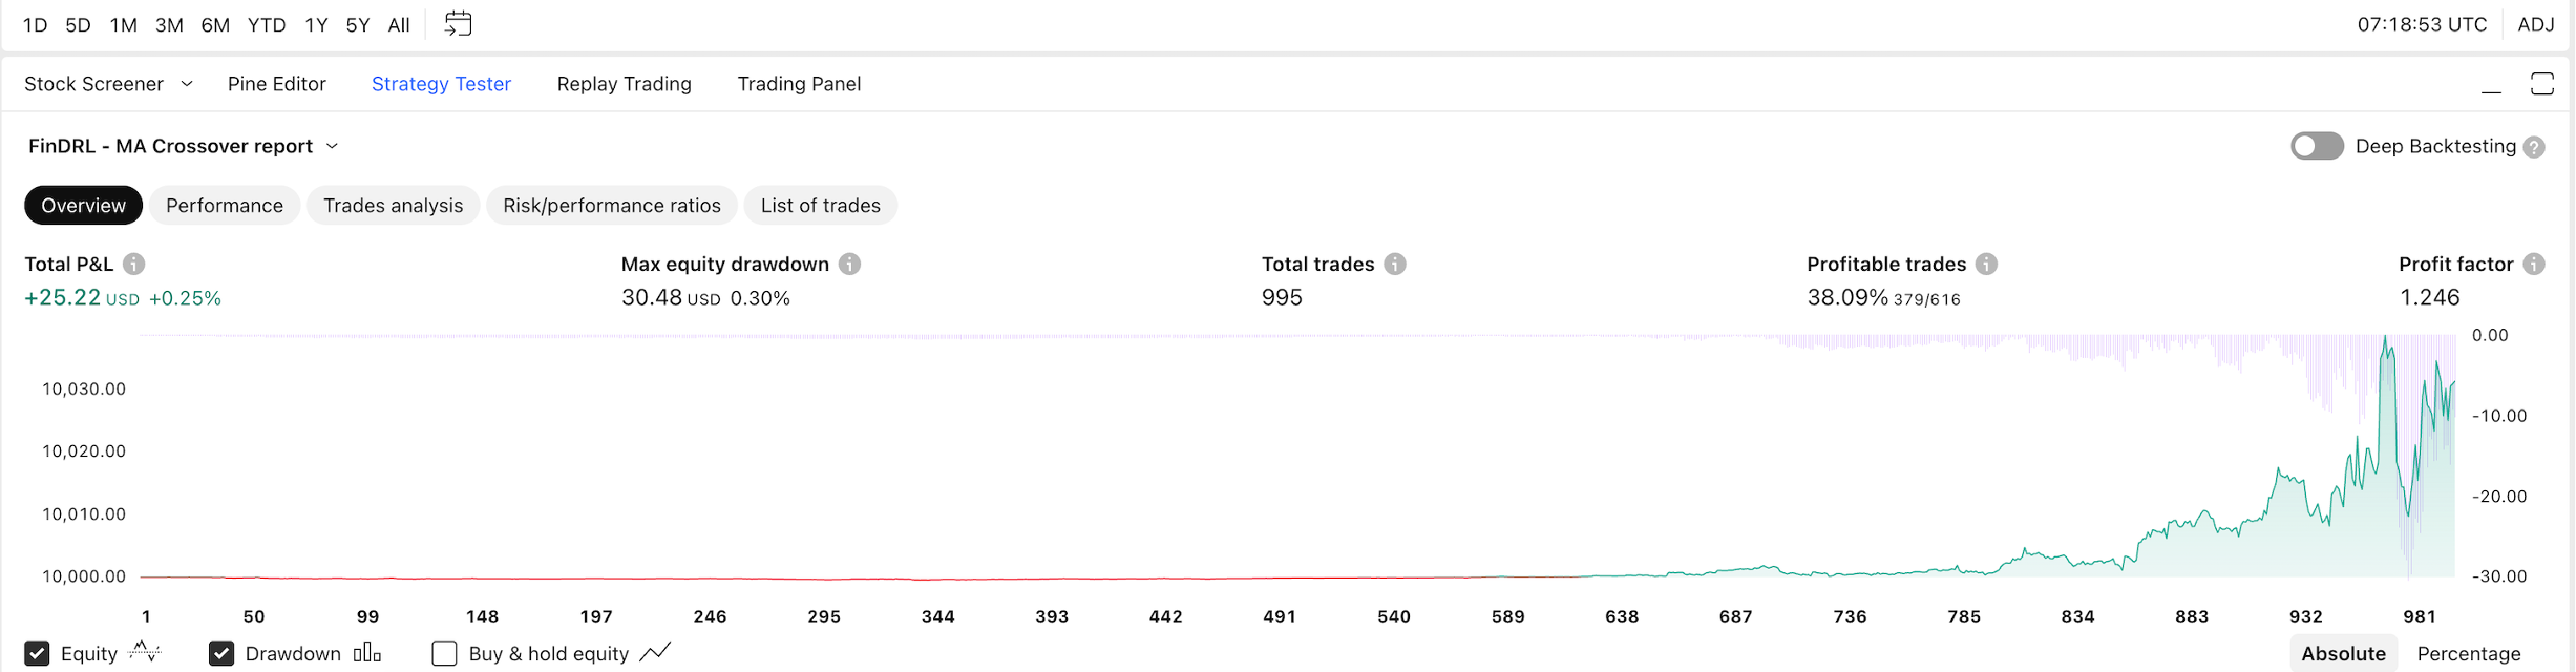
\includegraphics[width=.85\textwidth, height=3.6cm]{2-FinDRL-MA-Crossover}
        \caption{MA Crossover Strategy Performance}
        \label{fig:ma_performance}
    \end{figure}

    
    \item \textbf{FinDRL - MACD}: This strategy finds momentum shifts by calculating the distance between fast and slow exponential moving averages (EMA). The analysis of performance references the efficient and balanced nature of the strategy.On a more specific note that will be visible in the charts below, this strategy uses MACD (with periods 12, 26, 9), where it enters above the signal line - further confirmed by using \%K > \%D, where MACD = (EMA(12) - EMA(26)) and Signal = (EMA(MACD, 9). August 1, 2024 to February 26, 2015 1D NVDA Performance report- +27.69 USD(+0.28\%),960 Trades,37.60\% Win rate,24.83 USD DD,1.287 PF
    
    \begin{figure}[htbp]
        \centering
        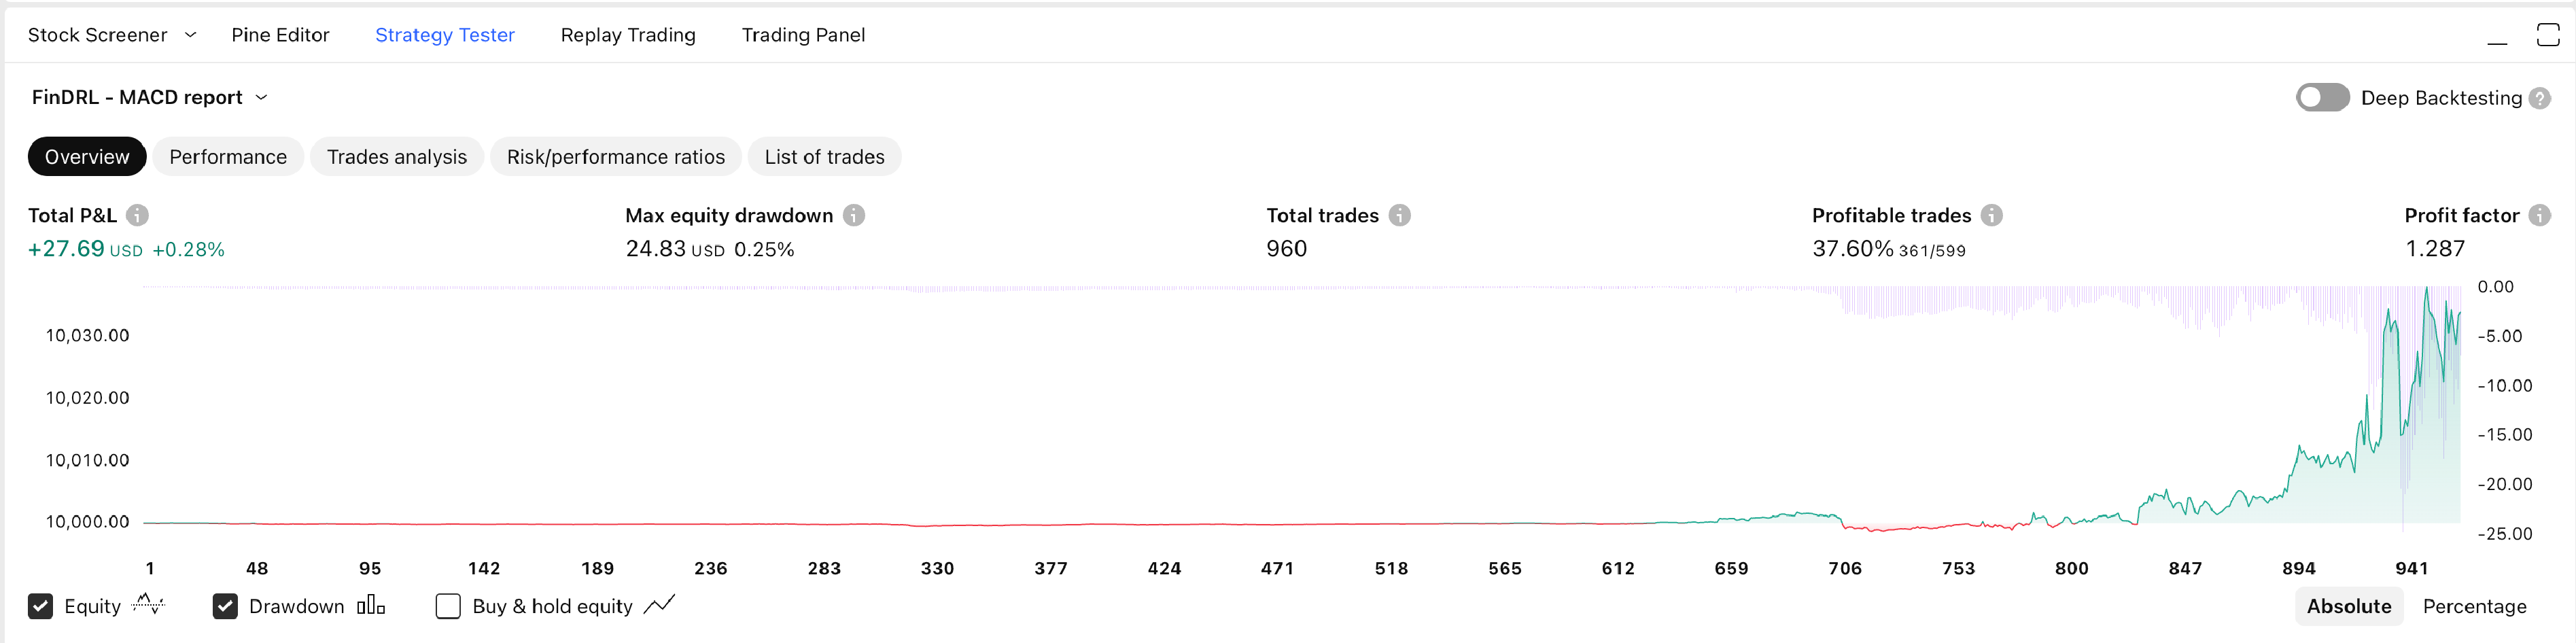
\includegraphics[width=.85\textwidth, height=3.6cm]{6-FinDRL-MACD}
        \caption{MA Crossover Strategy Performance}
        \label{fig:MACD performance}
    \end{figure}

    \item \textbf{FinDRL - Parabolic SAR}: Parabolic SAR strategy uses Parabolic Stop and Reverse (SAR) technical indicator, that creates set of trailing stop levels, by drawing the dots on price charts based on price acceleration. The Parabolic SAR with a starting acceleration of 0.02, increment of 0.02, and a maximum of 0.2 to observe pricing trends, entering the market on price emerging above SAR, with \%K crossing over \%D. SAR =(\text{Prev SAR}+\text{AF}*(\text{EP}-\text{Prev SAR})). Backtesting from August 1, 2024, to February 26, 2025 ↑922.0 ↓−9.89 USD (−0.10\%) ↑869 trades ↑39.24\% win rate ↑−26.64 USD do λ of return 0.965.
    
    \begin{figure}[htbp]
        \centering
        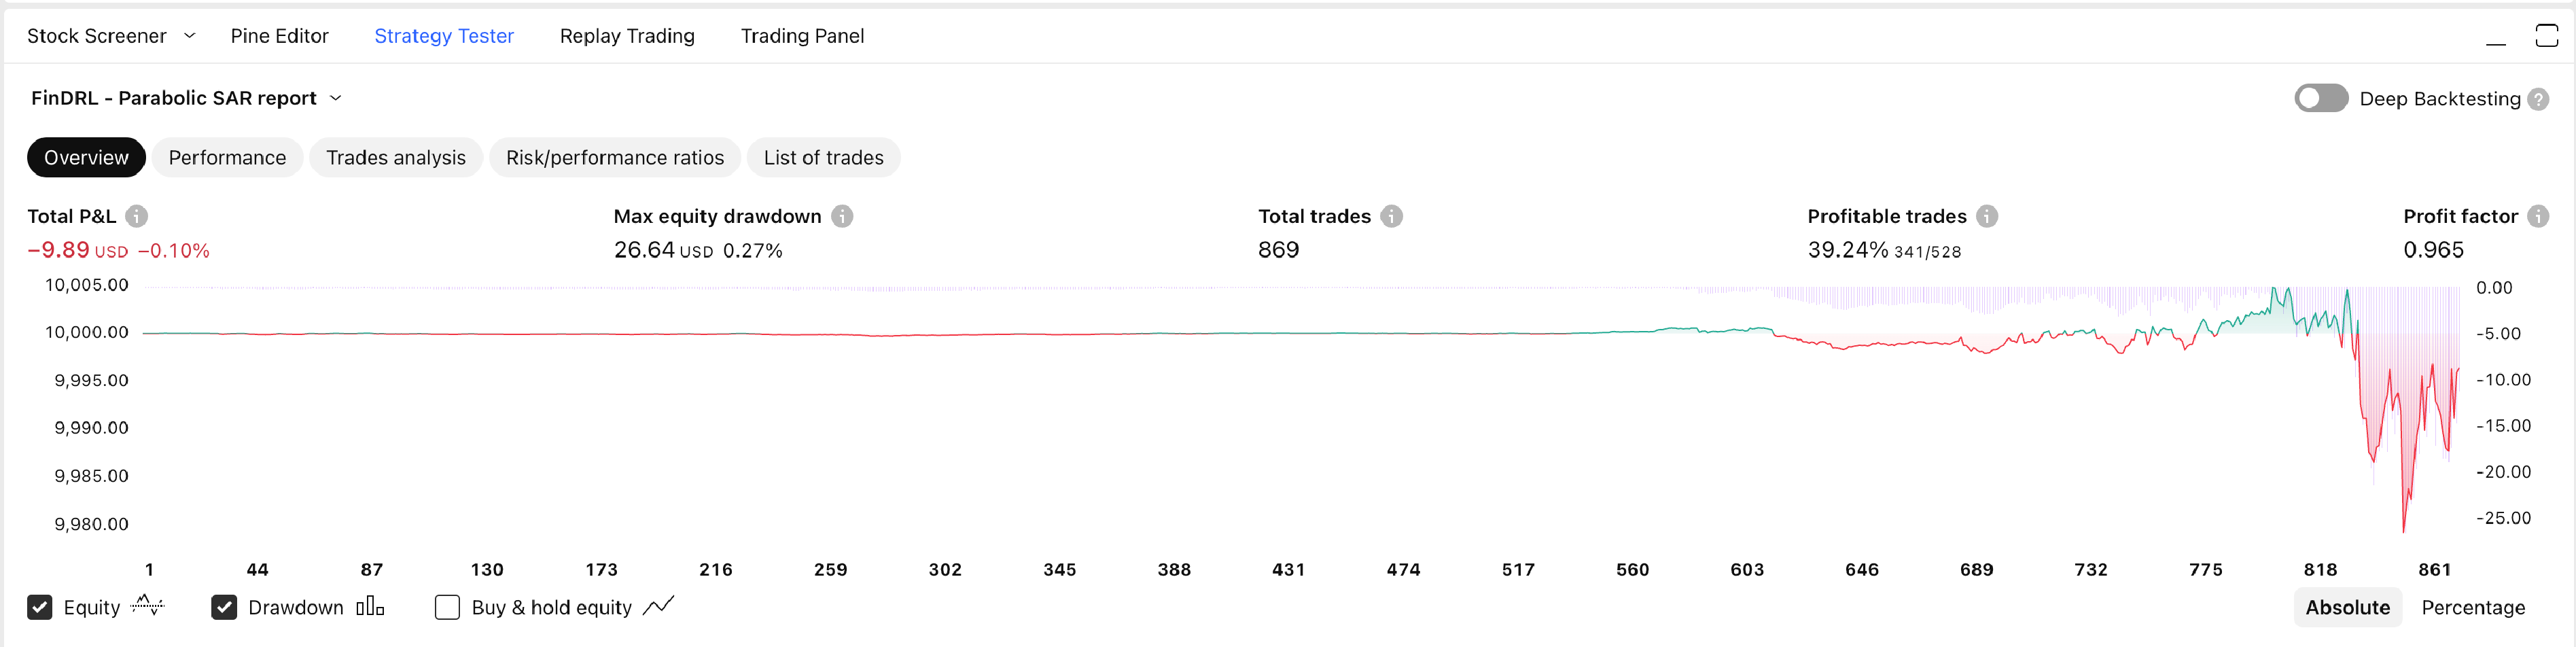
\includegraphics[width=.85\textwidth, height=3.6cm]{4-FinDRL-Parabolic-SAR}
        \caption{Parabolic SAR Strategy Performance}
        \label{fig:Parabolic SAR performance}
    \end{figure}

    \item \textbf{FinDRL - SuperTrend}: SuperTrend is a strategy where we use the SuperTrend feature which is derived from the Average True Range (ATR) combined with the mid-price (the average of the high and low) to form a moving average that attempts to capture the direction of the price movement. Employing a 10-period ATR with a factor of 3, this strategy enters on a bullish direction ($< 0$) when $\%K$ crosses 20, using adaptive band logic. Performance on 1D NVDA from July 1\, 2024\, to February 26\, 2025\, yielded +5.02 USD (+0.05\%), 266 trades, 36.09\% win rate, 15.78 USD drawdown, and a profit factor of 1.202.


    \begin{figure}[htbp]
        \centering
        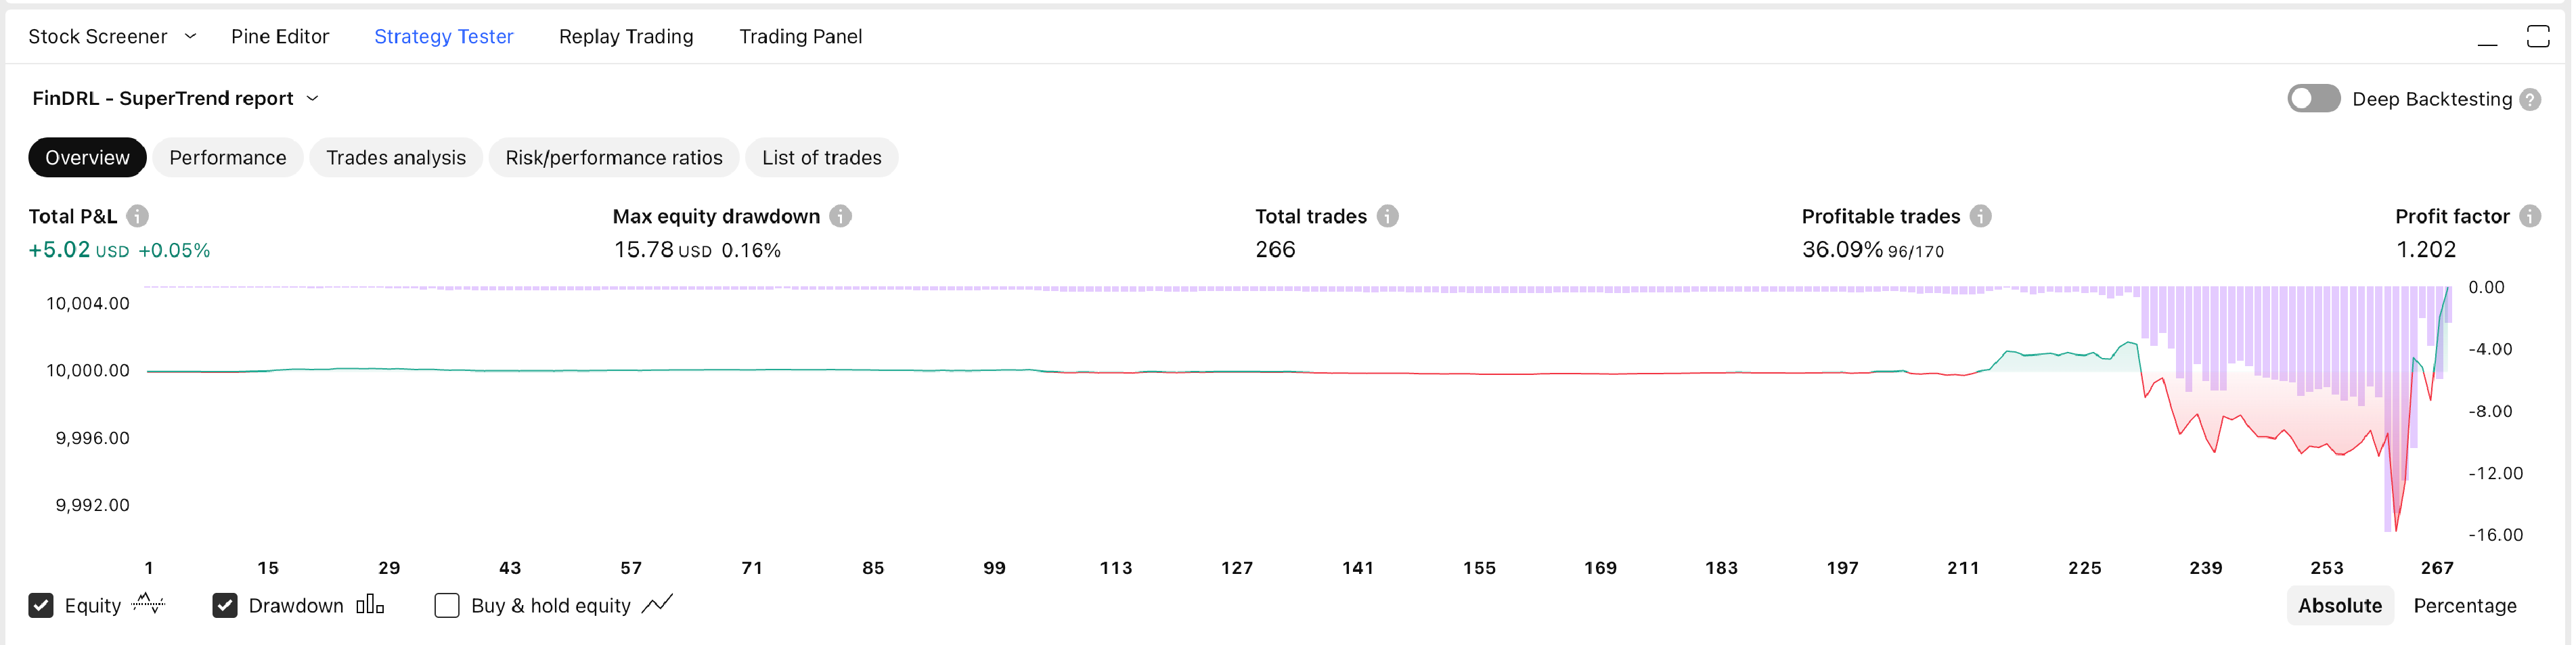
\includegraphics[width=.85\textwidth, height=3.6cm]{13-FinDRL-SuperTrend}
        \caption{SuperTrend Strategy Performance}
        \label{fig:SuperTrend performance}
    \end{figure}
    
    \item \textbf{FinDRL - Momentum}: This strategy measures 10-period momentum, entering when > 0 and \%K is rising, with Momentum = \(\text{close} - \text{close}[10]\). Backtesting from August 1, 2024, to February 26, 2025, resulted in +38.62 USD (+0.39\%), 1,065 trades, 36.81\% win rate, 36.29 USD drawdown, and a profit factor of 1.257.
    
    \begin{figure}[htbp]
        \centering
        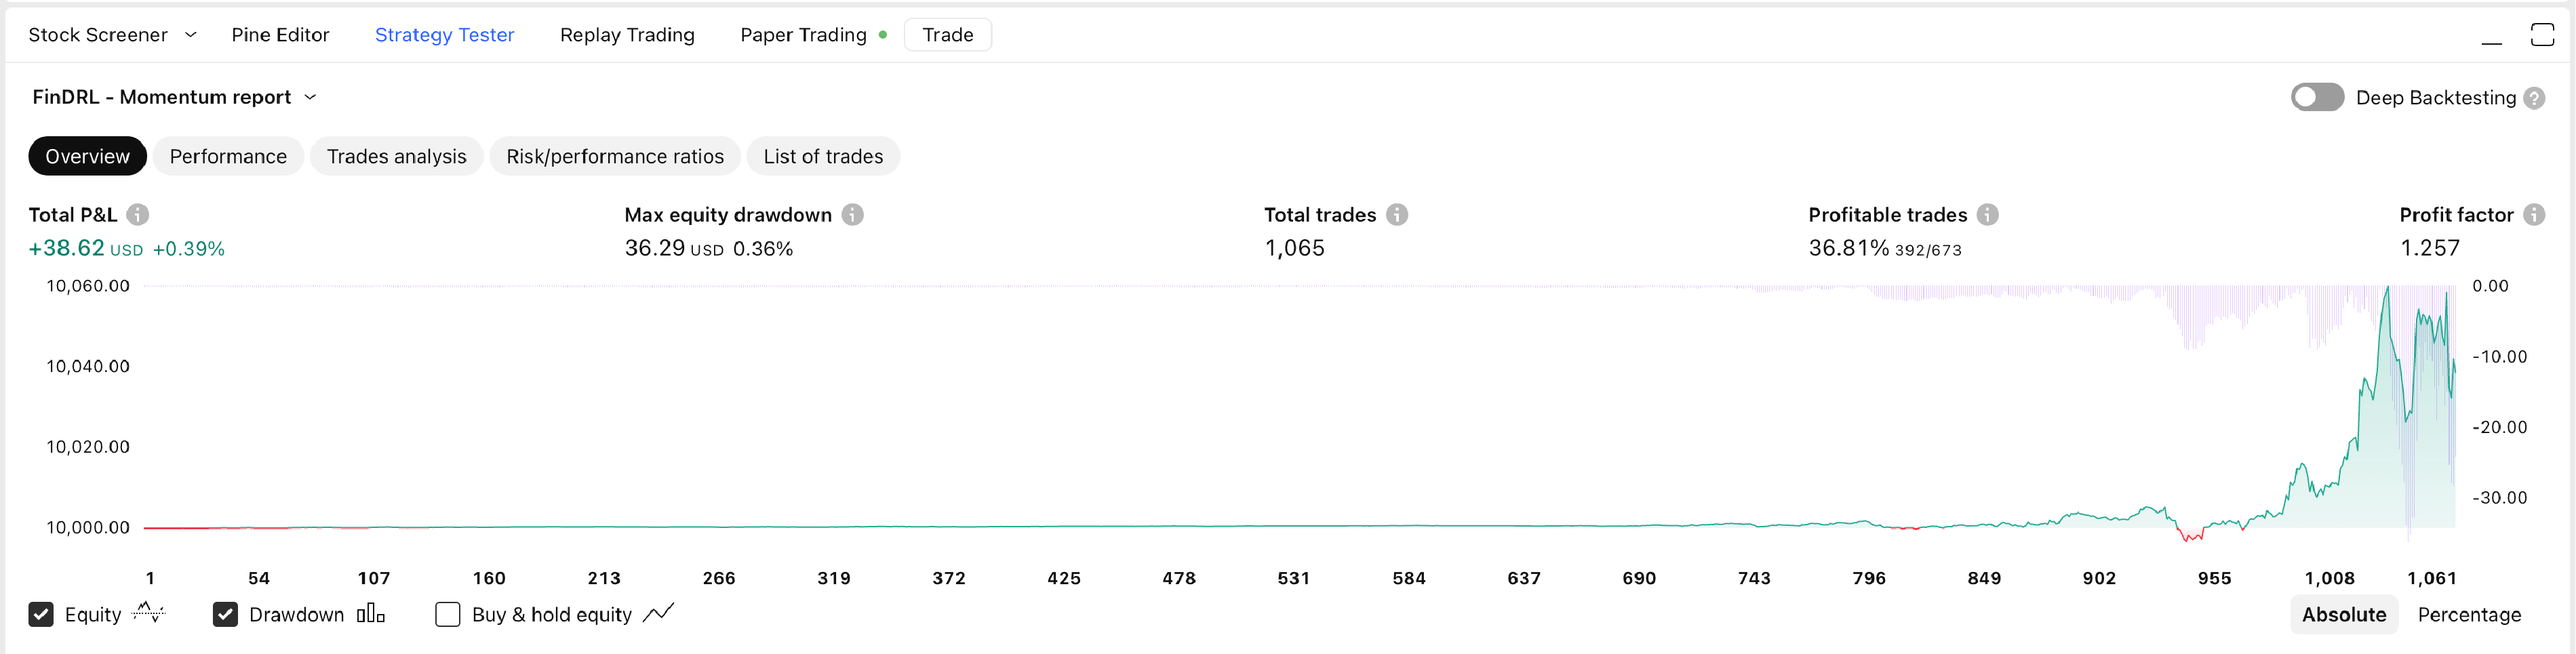
\includegraphics[width=.85\textwidth, height=3.6cm]{17-FinDRL-Momentum}
        \caption{MA Crossover Strategy Performance}
        \label{fig:momentum_performance}
    \end{figure}
    
    \item \textbf{FinDRL - Ichimoku Cloud}: Incorporating Tenkan (9), Kijun (26), and Senkou Span A/B (52), this strategy enters when the price exceeds both Span A and Span B, with \%K > 50. The equations are Span A = \((\text{Tenkan} + \text{Kijun}) / 2\) and Span B = \((\text{highest(high, 52)} + \text{lowest(low, 52)}) / 2\). Performance from July 1, 2024, to February 26, 2025, showed +20.03 USD (+0.20\%), 330 trades, 31.82\% win rate, 69.96 USD drawdown, and a profit factor of 1.218.

    \begin{figure}[htbp]
        \centering
        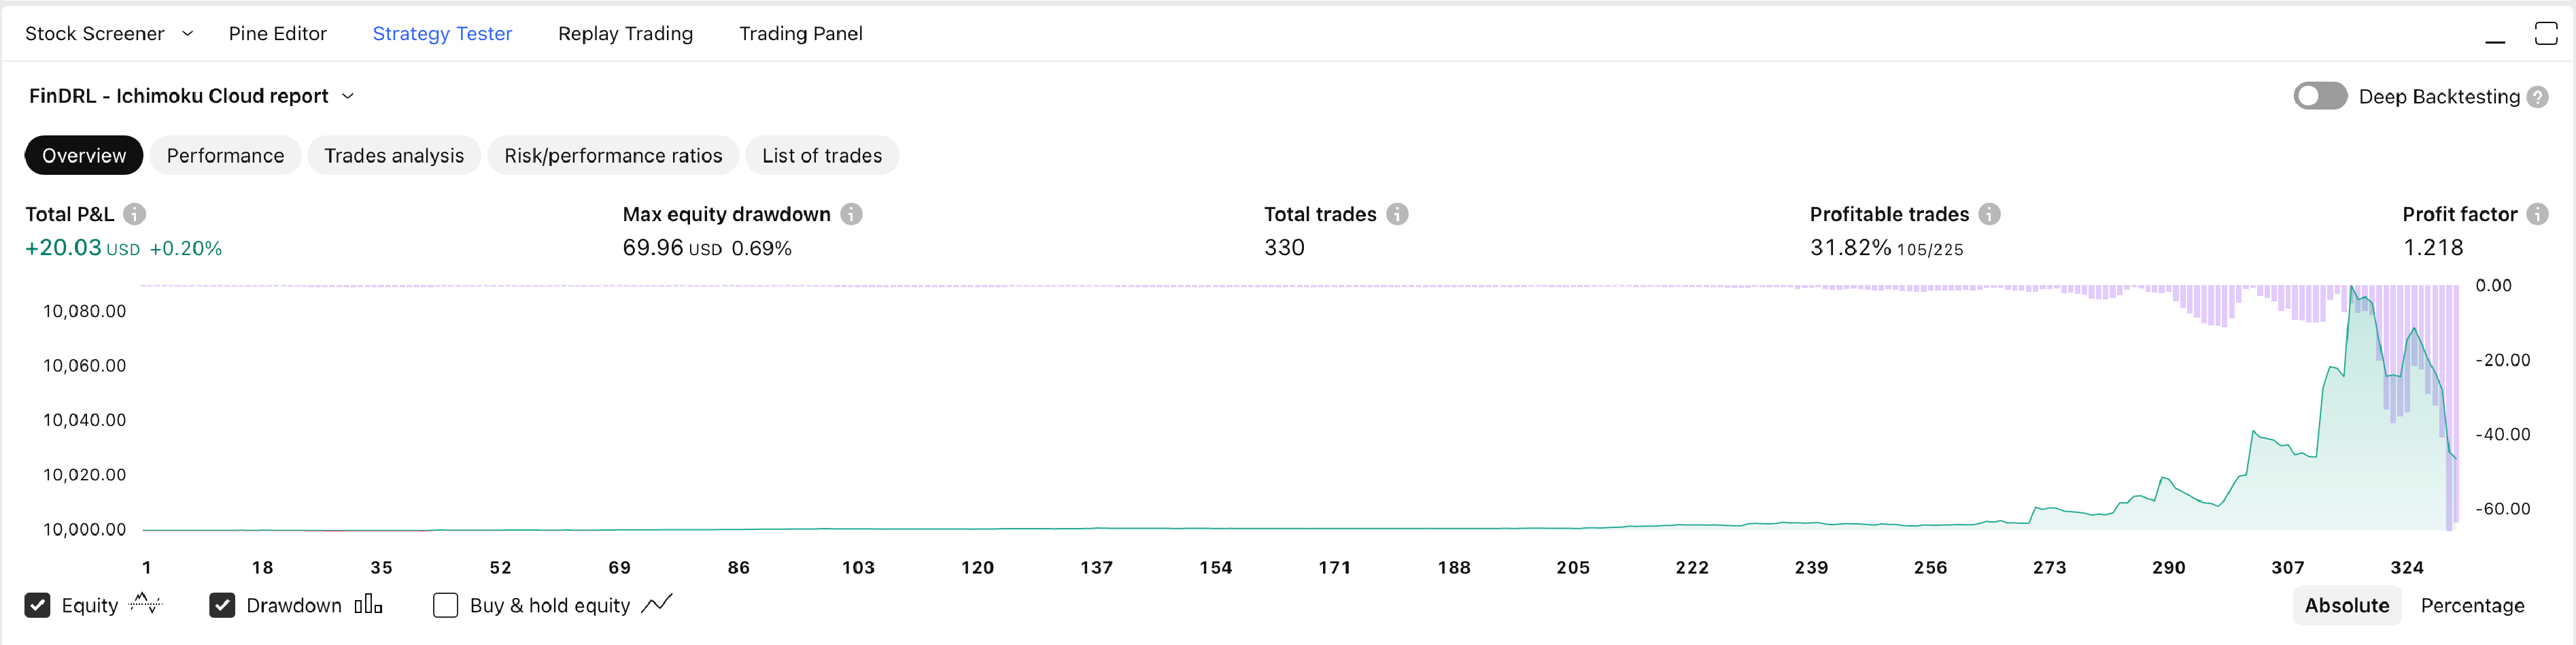
\includegraphics[width=.85\textwidth, height=3.6cm]{5-FinDRL-Ichimoku-Cloud}
        \caption{Ichimoku Cloud Strategy Performance}
        \label{fig: ichimoku_cloud_performance}
    \end{figure}
    
    \item \textbf{FinDRL - ADX}: This strategy enters when ADX > 25 and \%K > \%D, quantifying trend strength with ADX = \(\text{SMA}(\text{abs}(\text{DI+} - \text{DI-}) / (\text{DI+} + \text{DI-}), 14)\). Backtesting from August 1, 2024, to February 26, 2025, yielded +32.74 USD (+0.33\%), 887 trades, 33.71\% win rate, 50.43 USD drawdown, and a profit factor of 1.253.

    \begin{figure}[htbp]
        \centering
        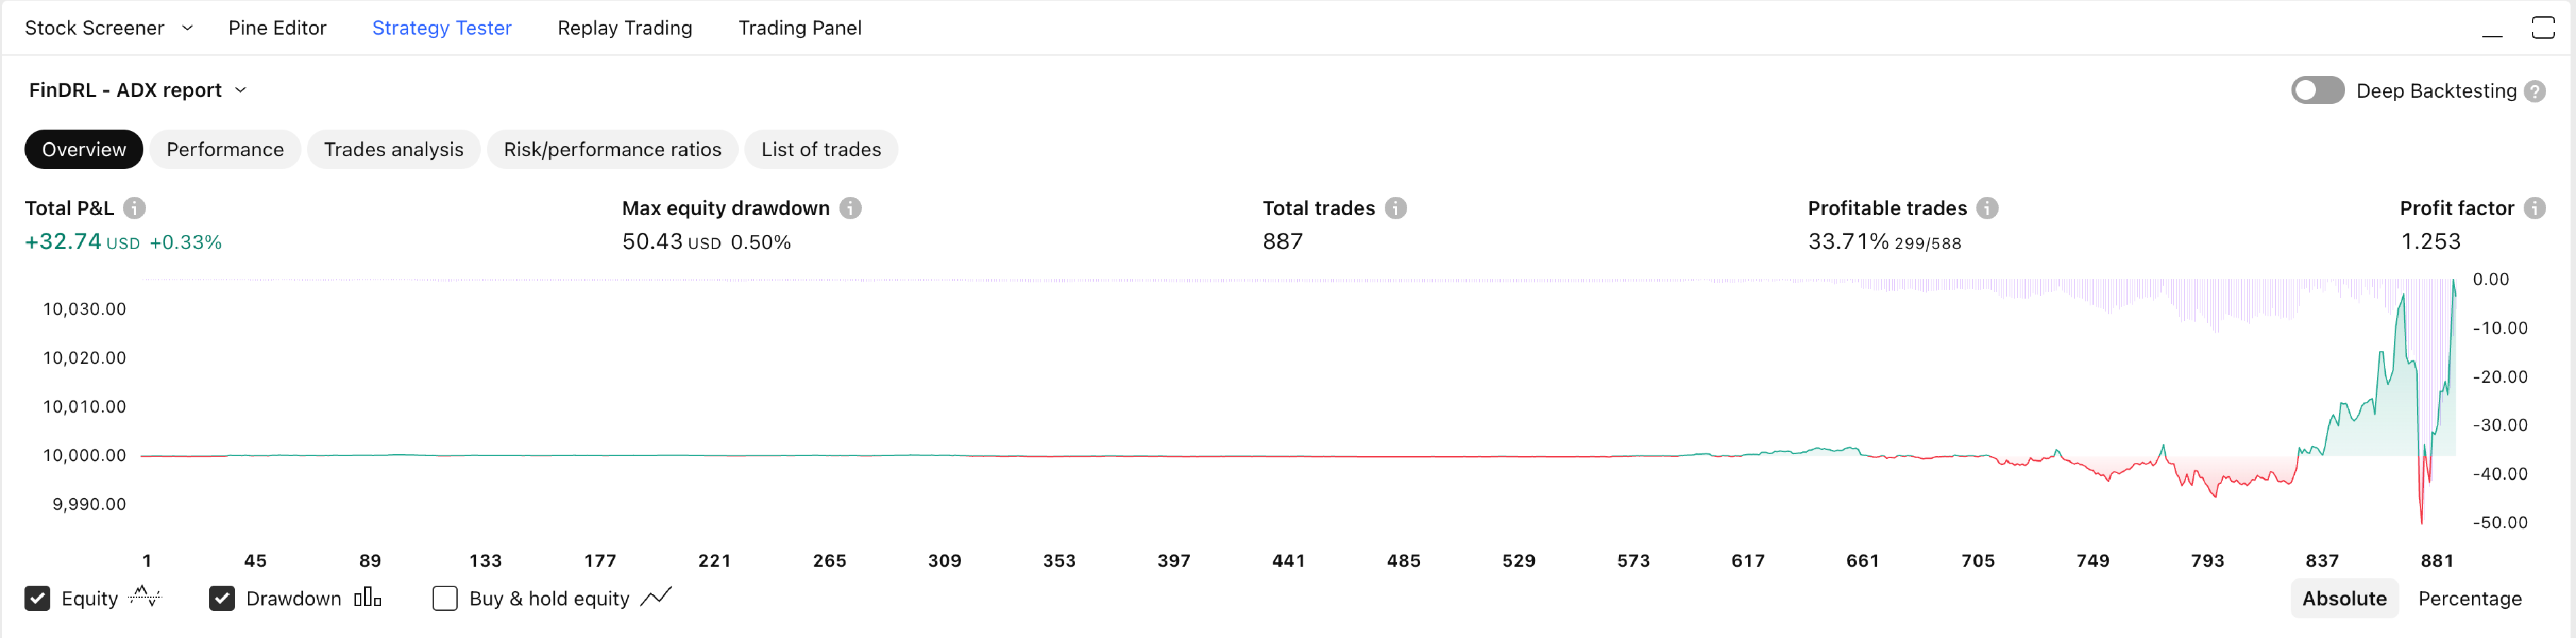
\includegraphics[width=.85\textwidth, height=3.6cm]{8-FinDRL-ADX}
        \caption{ADX Strategy Performance}
        \label{fig:adx_performance}
    \end{figure}
    
\end{itemize}
These strategies perform exceptionally in trending markets, with FinDRL - Momentum and FinDRL - MACD leading in profitability, though FinDRL - Parabolic SAR struggled, possibly due to market choppiness.

\subsection{Breakout Strategies}
\begin{itemize}
    \item \textbf{FinDRL - Gaussian Channel}: Enters when the price exceeds \(\text{mean} + 2 \times \sigma\) over a 20-period SMA, with \%K > \%D. The mathematical basis includes Mean = \(\frac{\sum \text{close}}{20}\) and \(\sigma = \sqrt{\frac{\sum (\text{close} - \text{mean})^2}{20}}\). Backtesting on 1D NVDA from January 1, 2023, to November 14, 2025, resulted in +2.29 USD (+0.02\%), 236 trades, 38.98\% win rate, 10.19 USD drawdown, and a profit factor of 1.105.

    \begin{figure}[htbp]
        \centering
        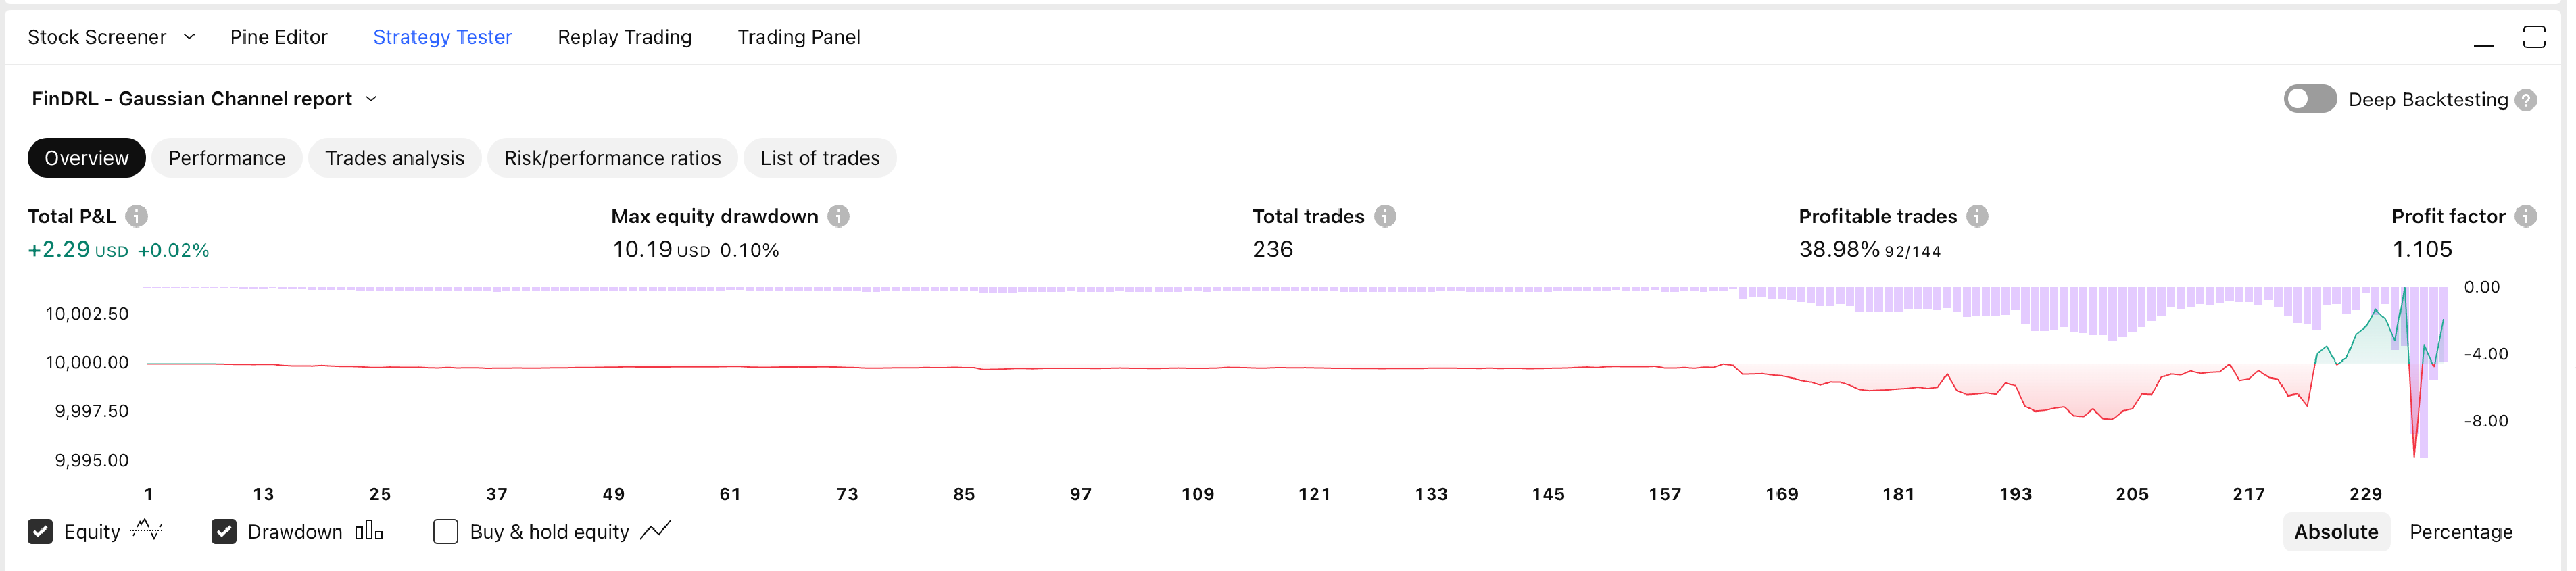
\includegraphics[width=.85\textwidth, height=3.6cm]{1-FinDRL-Gaussian-Channel}
        \caption{Gaussian Channel Strategy Performance}
        \label{fig:gaussian_channel_performance}
    \end{figure}
    
    \item \textbf{FinDRL - Bollinger Bands}: Enters when the price surpasses \(\text{SMA} + 2 \times \sigma\) over 20 periods, with \%K > 20. The calculation uses SMA = \(\frac{\sum \text{close}}{20}\) and \(\sigma = \sqrt{\frac{\sum (\text{close} - \text{SMA})^2}{20}}\). Performance from July 1, 2024, to February 26, 2025, showed -0.78 USD (-0.01\%), 251 trades, 35.06\% win rate, 13.16 USD drawdown, and a profit factor of 0.975.

    \begin{figure}[htbp]
        \centering
        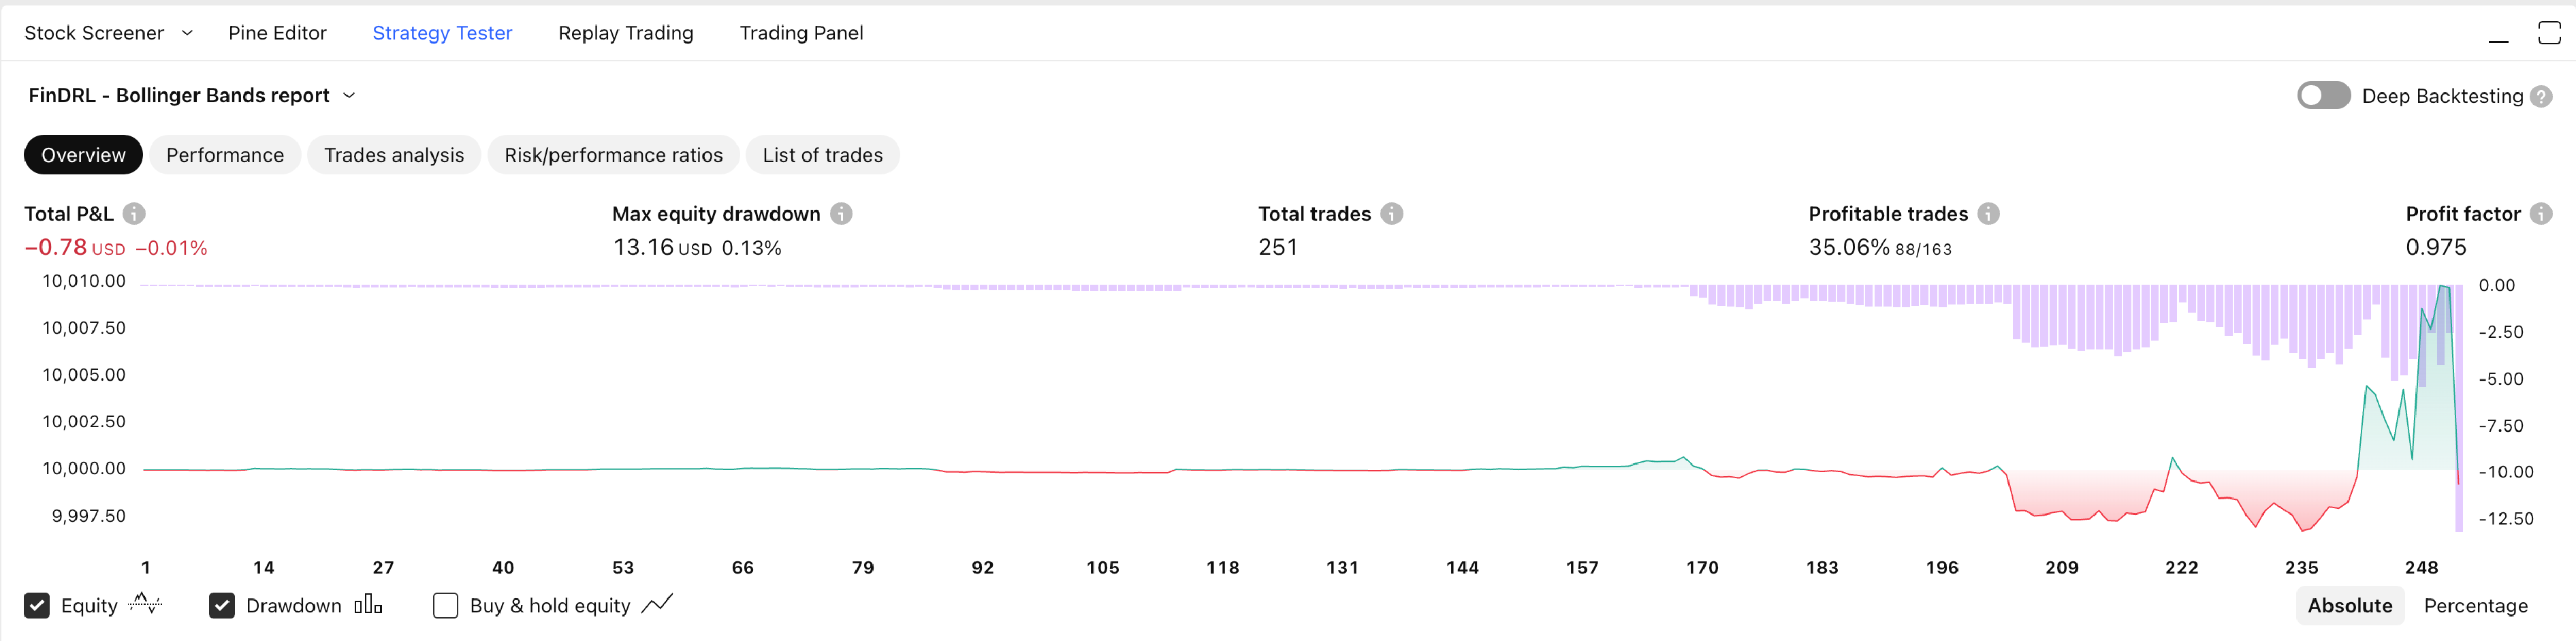
\includegraphics[width=.85\textwidth, height=3.6cm]{3-FinDRL-Bollinger-Bands}
        \caption{Parabolic SAR Strategy Performance}
        \label{fig:bollinger_bands_performance}
    \end{figure}
    
    \item \textbf{FinDRL - Donchian Channel}: Enters when the price exceeds the highest high over 20 periods, with \%K > 20, where Upper = \(\text{max(high, 20)}\). Backtesting from September 1, 2024, to February 26, 2025, resulted in 0 USD (0.00\%), 0 trades, 0\% win rate, and a profit factor of NA.

    \begin{figure}[htbp]
        \centering
        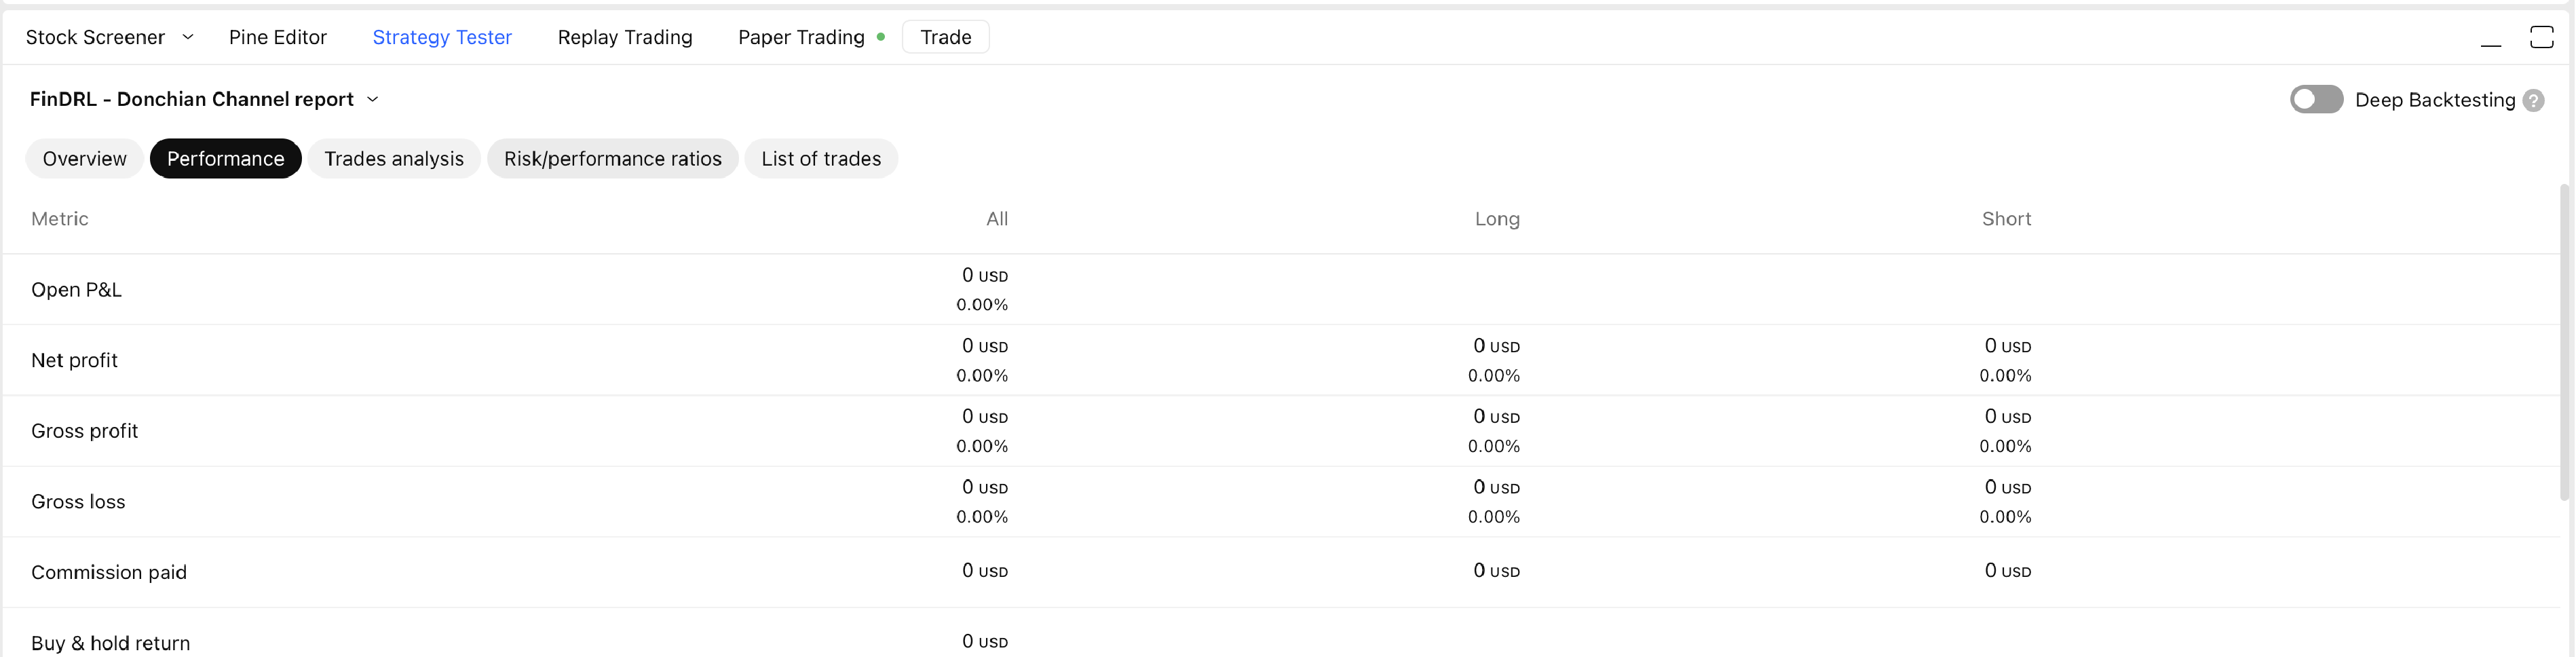
\includegraphics[width=.85\textwidth, height=3.6cm]{11-FinDRL-Donchian-Channel}
        \caption{Donchian Channel Strategy Performance}
        \label{fig:Donchian Channel performance}
    \end{figure}
    
    \item \textbf{FinDRL - Keltner Channel}: Enters when the price exceeds \(\text{EMA} + 2 \times \text{ATR}\) over 20 periods, with \%K > \%D. The equations are EMA = \(\text{EMA}(\text{close}, 20)\) and ATR = \(\text{SMA}(\text{TR}, 20)\). Performance from July 1, 2024, to February 26, 2025, yielded +7.19 USD (+0.07\%), 301 trades, 38.54\% win rate, 21.18 USD drawdown, and a profit factor of 1.165.

    \begin{figure}[htbp]
        \centering
        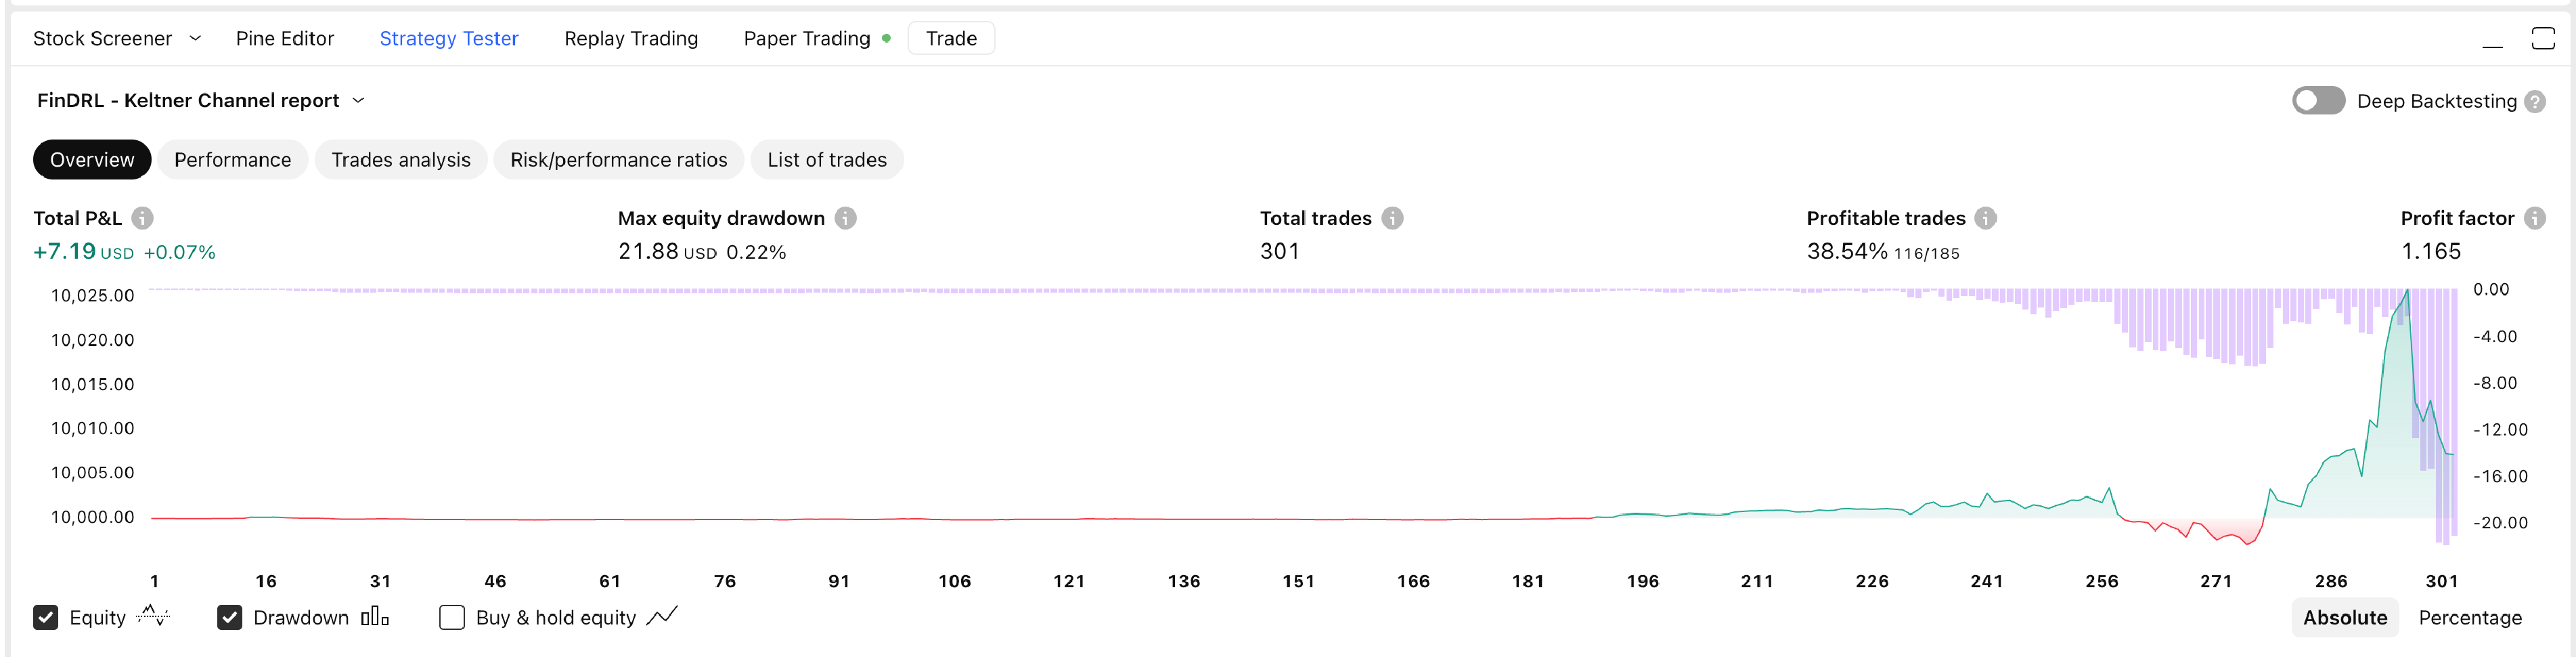
\includegraphics[width=.85\textwidth, height=3.6cm]{12-FinDRL-Keltner-Channel}
        \caption{Keltner Channel Strategy Performance}
        \label{fig:Keltner Channel performance}
    \end{figure}
    
    \item \textbf{FinDRL - ATR}: Enters when the price exceeds \(\text{close} + \text{ATR}(14)\), with \%K rising. The formula is ATR = \(\text{SMA}(\text{max(high} - \text{low}, \text{abs(high} - \text{close}[1]), \text{abs(low} - \text{close}[1])), 14)\). Backtesting from September 1, 2025, to February 26, 2025, showed 0 USD (0.00\%), 0 trades, 0\% win rate, and a profit factor of NA.

    \begin{figure}[htbp]
        \centering
        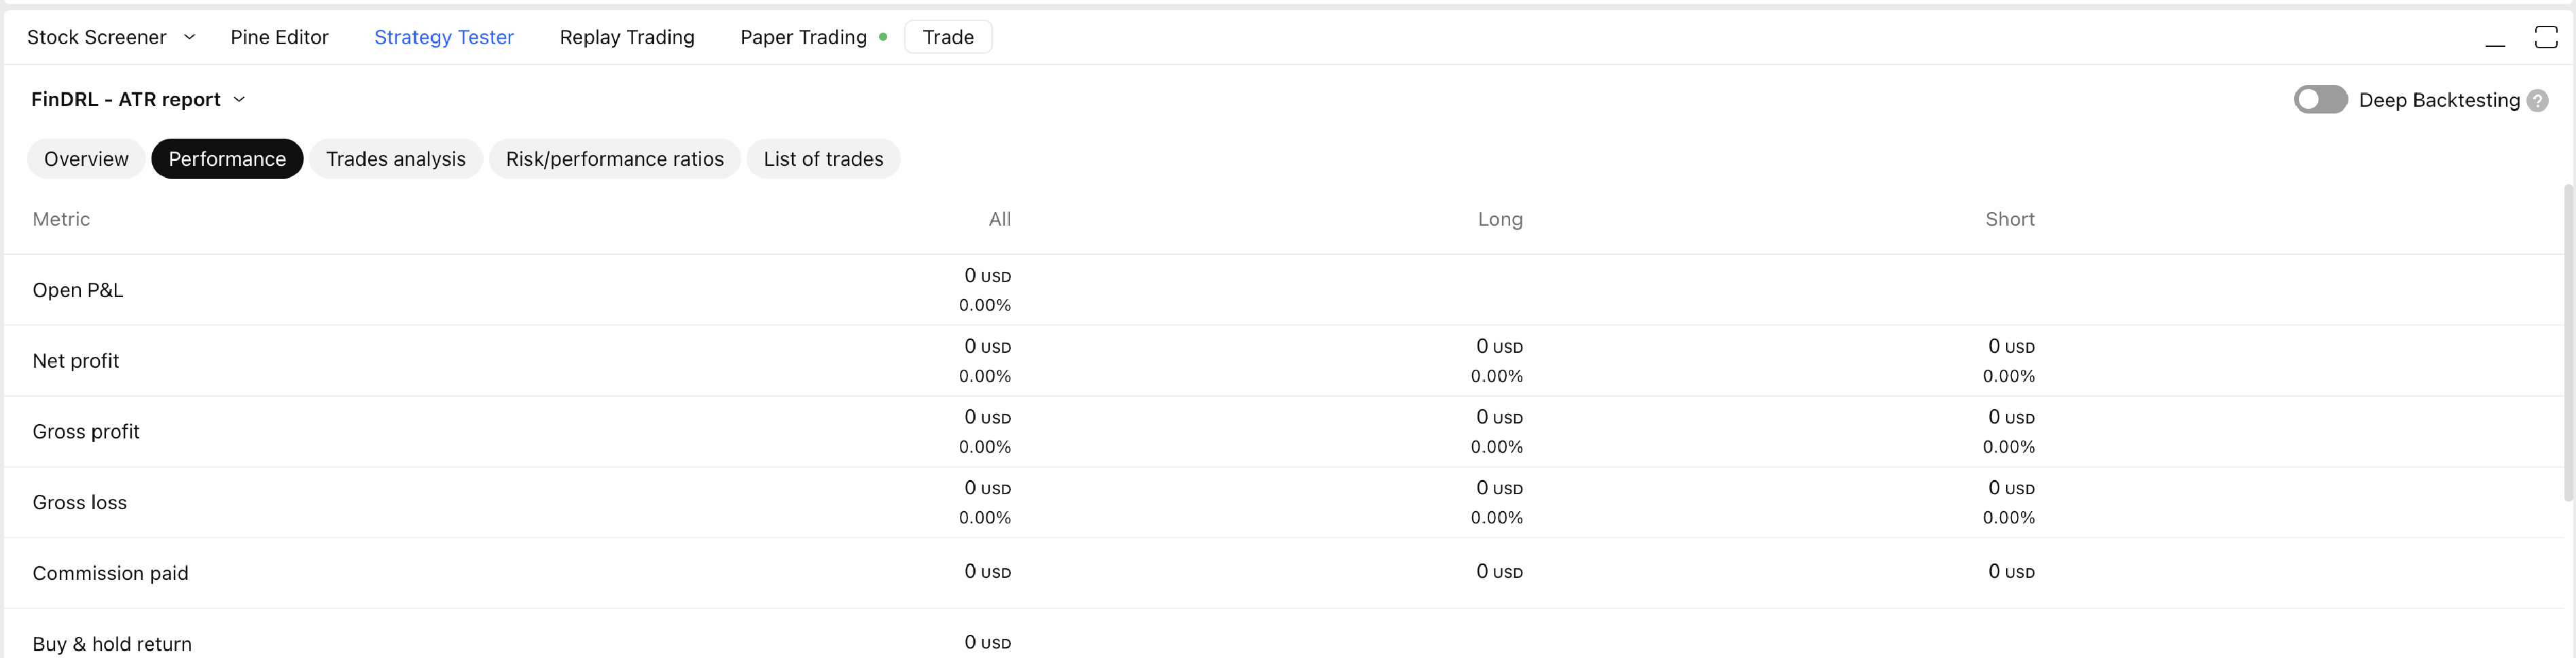
\includegraphics[width=.85\textwidth, height=3.6cm]{9-FinDRL-ATR}
        \caption{ATR Strategy Performance}
        \label{fig:ATR performance}
    \end{figure}
    
    \item \textbf{FinDRL - Volume Spike}: Enters when volume > \(2 \times \text{SMA}(\text{volume}, 20)\), with \%K > \%D. The average volume is \(\frac{\sum \text{volume}}{20}\). Performance from August 15, 2024, to February 26, 2025, resulted in +7.69 USD (+0.08\%), 98 trades, 34.69\% win rate, 6.46 USD drawdown, and a profit factor of 2.469.

    \begin{figure}[htbp]
        \centering
        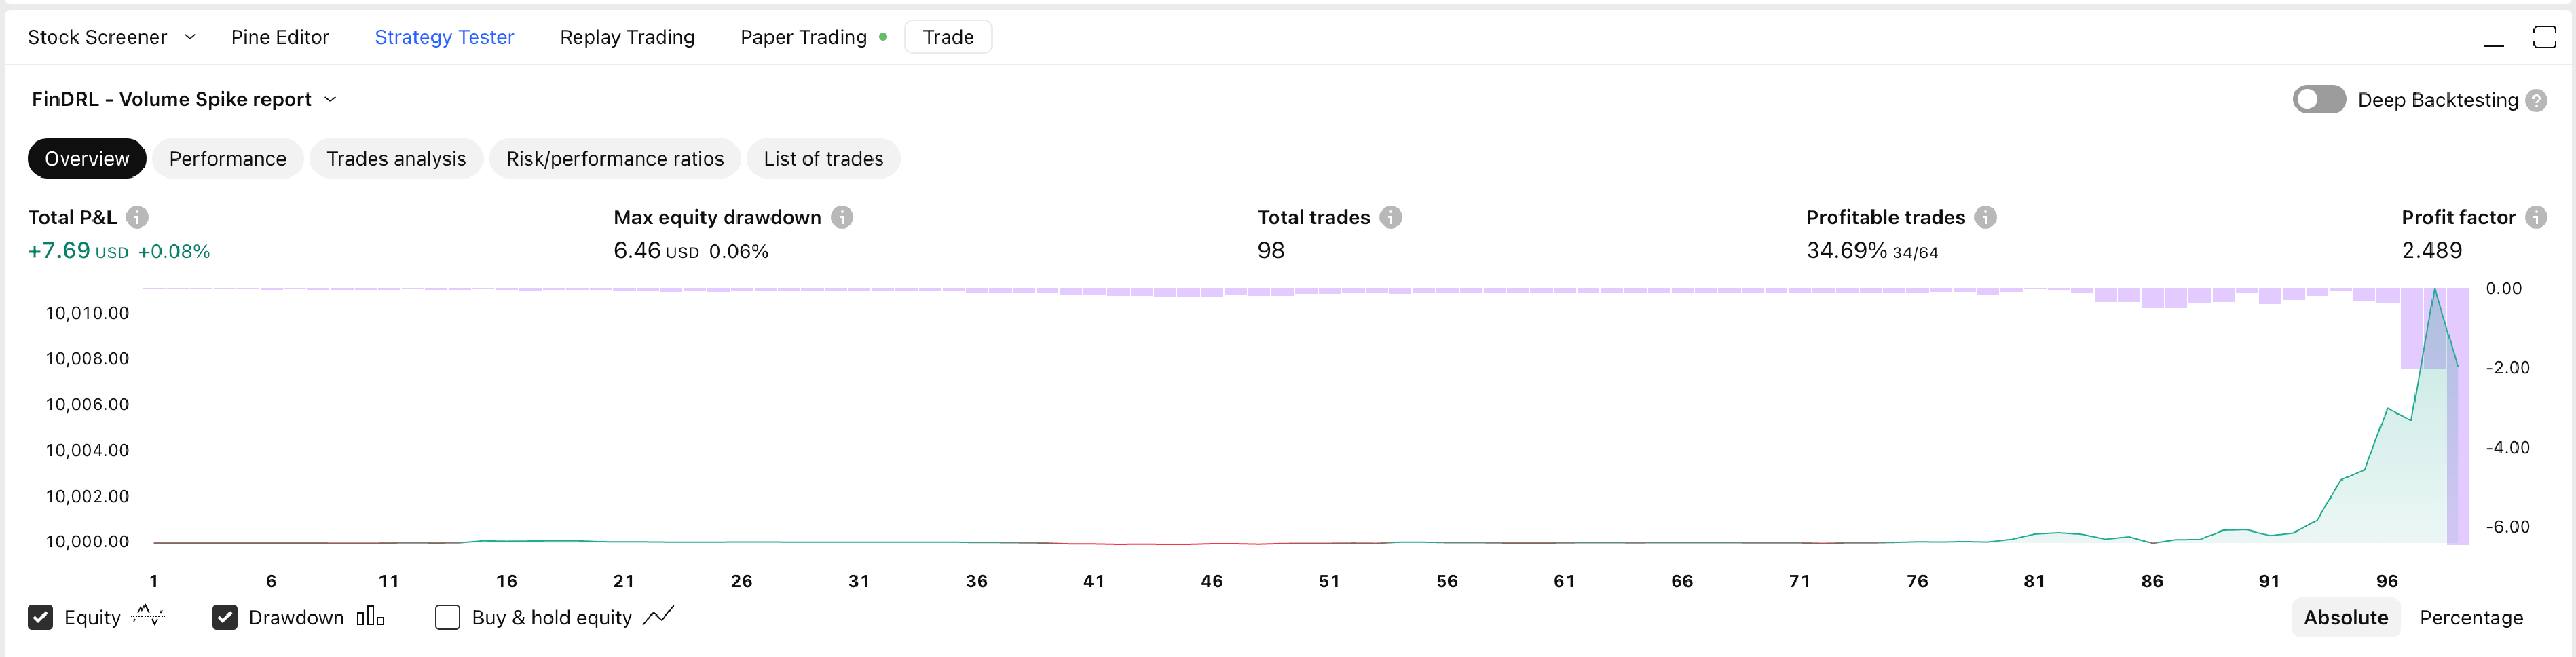
\includegraphics[width=.85\textwidth, height=3.6cm]{16-FinDRL-Volume-Spike}
        \caption{Volume Spike Strategy Performance}
        \label{fig:Volume Spike performance}
    \end{figure}
    
\end{itemize}
Breakout strategies exhibit varied success, with FinDRL - Volume Spike excelling due to its volume emphasis, while FinDRL - Donchian Channel and FinDRL - ATR failed to execute trades, suggesting possible configuration issues.

\subsection{Mean-Reversion Strategies}
\begin{itemize}

    \item \textbf{FinDRL - Stochastic RSI}: Enters when \%K < 20 and \%K crosses \%D. The \%K is \( \left( \frac{(\text{RSI} - \text{Min RSI})}{(\text{Max RSI} - \text{Min RSI})} \right) \times 100 \). Performance from September 15, 2009, to February 26, 2025, yielded +13.60 USD (+0.14\%), 284 trades, 33.80\% win rate, 9.32 USD drawdown, and a profit factor of 1.669.

    \begin{figure}[htbp]
        \centering
        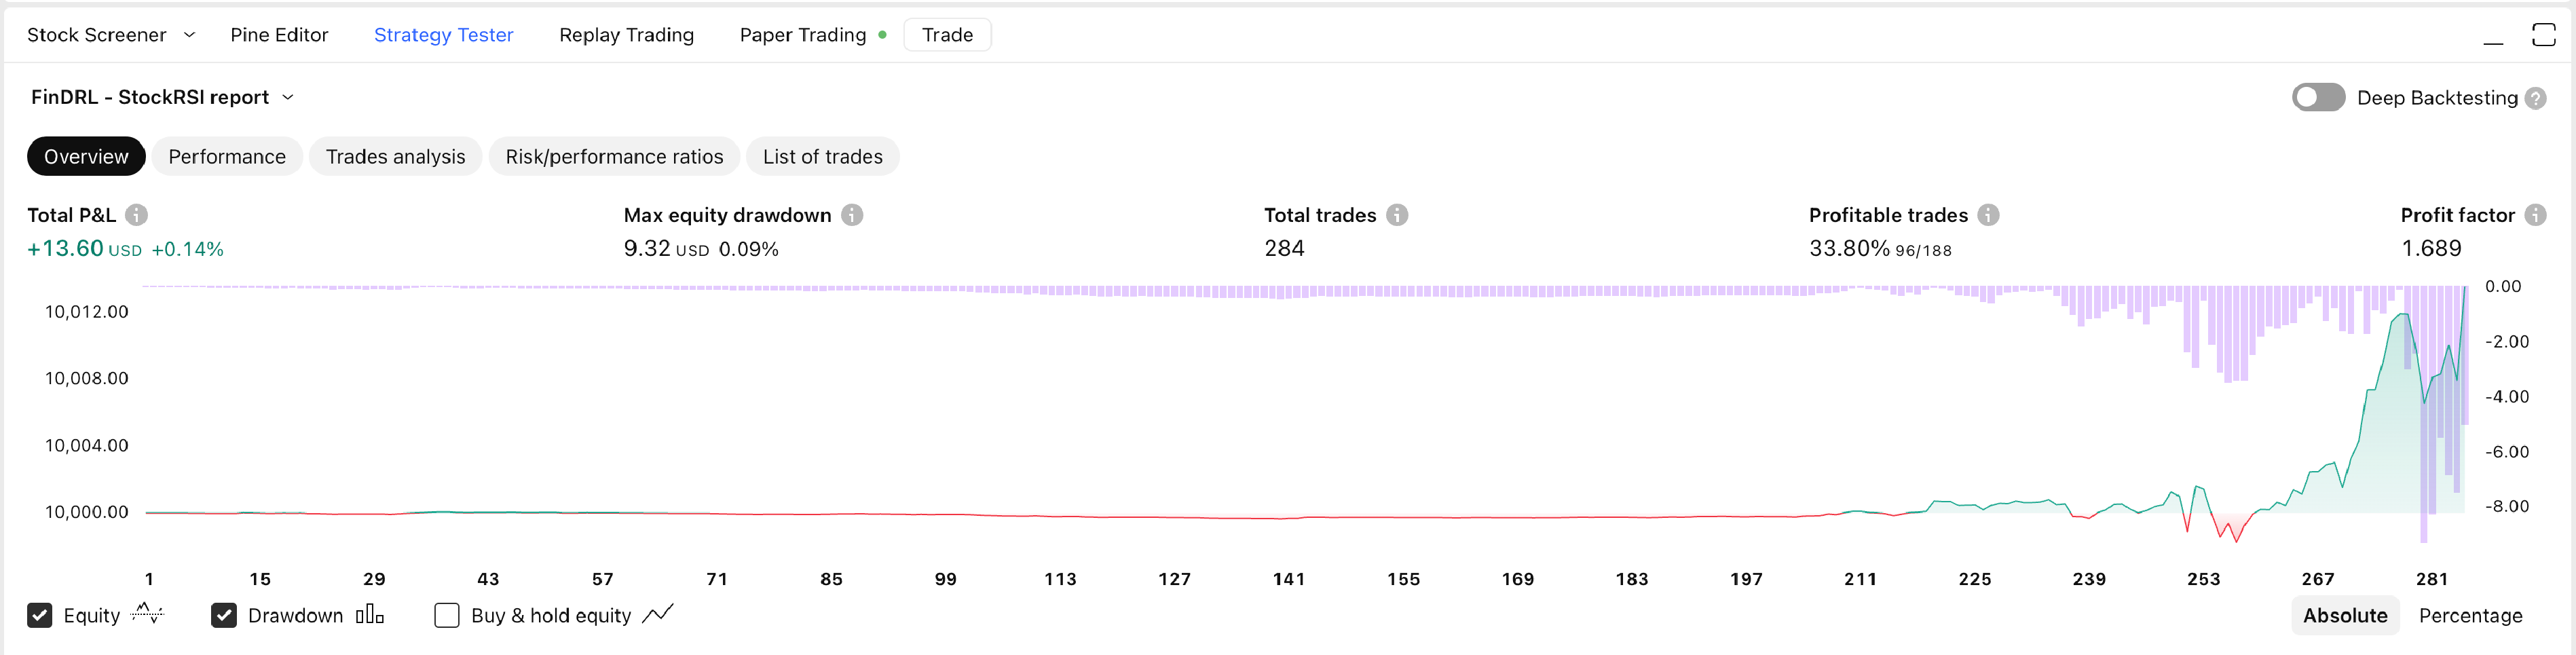
\includegraphics[width=.85\textwidth, height=3.6cm]{7-FinDRL-StockRSI}
        \caption{Stochastic Strategy Performance}
        \label{fig:Stochastic performance}
    \end{figure}

    \item \textbf{FinDRL - Williams \%R}: Enters when WillR < -80 and \%K crosses \%D. The WillR is \(((\text{max(high, 14)} - \text{close}) / (\text{max(high, 14)} - \text{min(low, 14}))) \times -100\). Backtesting from July 1, 2007, to February 26, 2025, showed +10.95 USD (+0.11\%), 184 trades, 29.89\% win rate, 7.10 USD drawdown, and a profit factor of 1.972.

    \begin{figure}[htbp]
        \centering
        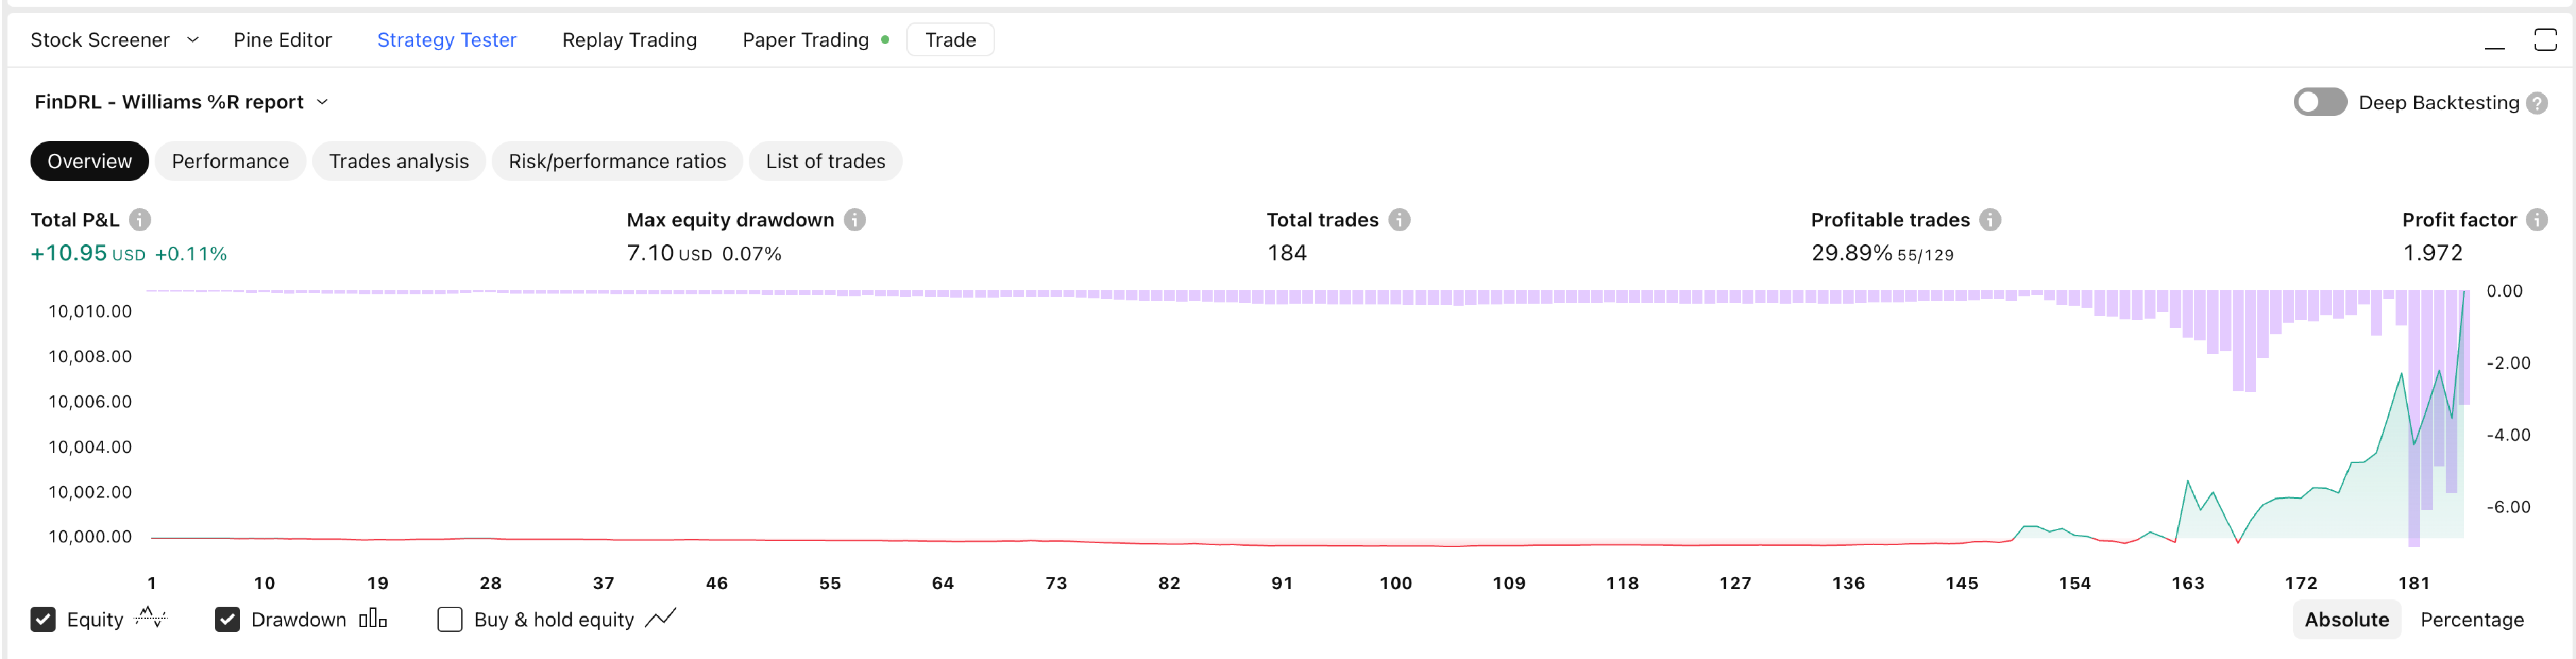
\includegraphics[width=.85\textwidth, height=3.6cm]{18-FinDRL-Williams-R}
        \caption{Williams \%R Strategy Performance}
        \label{fig:Williams R performance}
    \end{figure}
    
    \item \textbf{FinDRL - Fibonacci}: Enters when the price is within 5\% of the 61.8\% retracement level, with \%K > \%D. The Fib 61.8\% is \(\text{low} + 0.618 \times (\text{high} - \text{low})\). Performance from August 26, 2024, to February 26, 2025, resulted in +3.67 USD (+0.04\%), 211 trades, 35.55\% win rate, 11.47 USD drawdown, and a profit factor of 1.178.

    \begin{figure}[htbp]
        \centering
        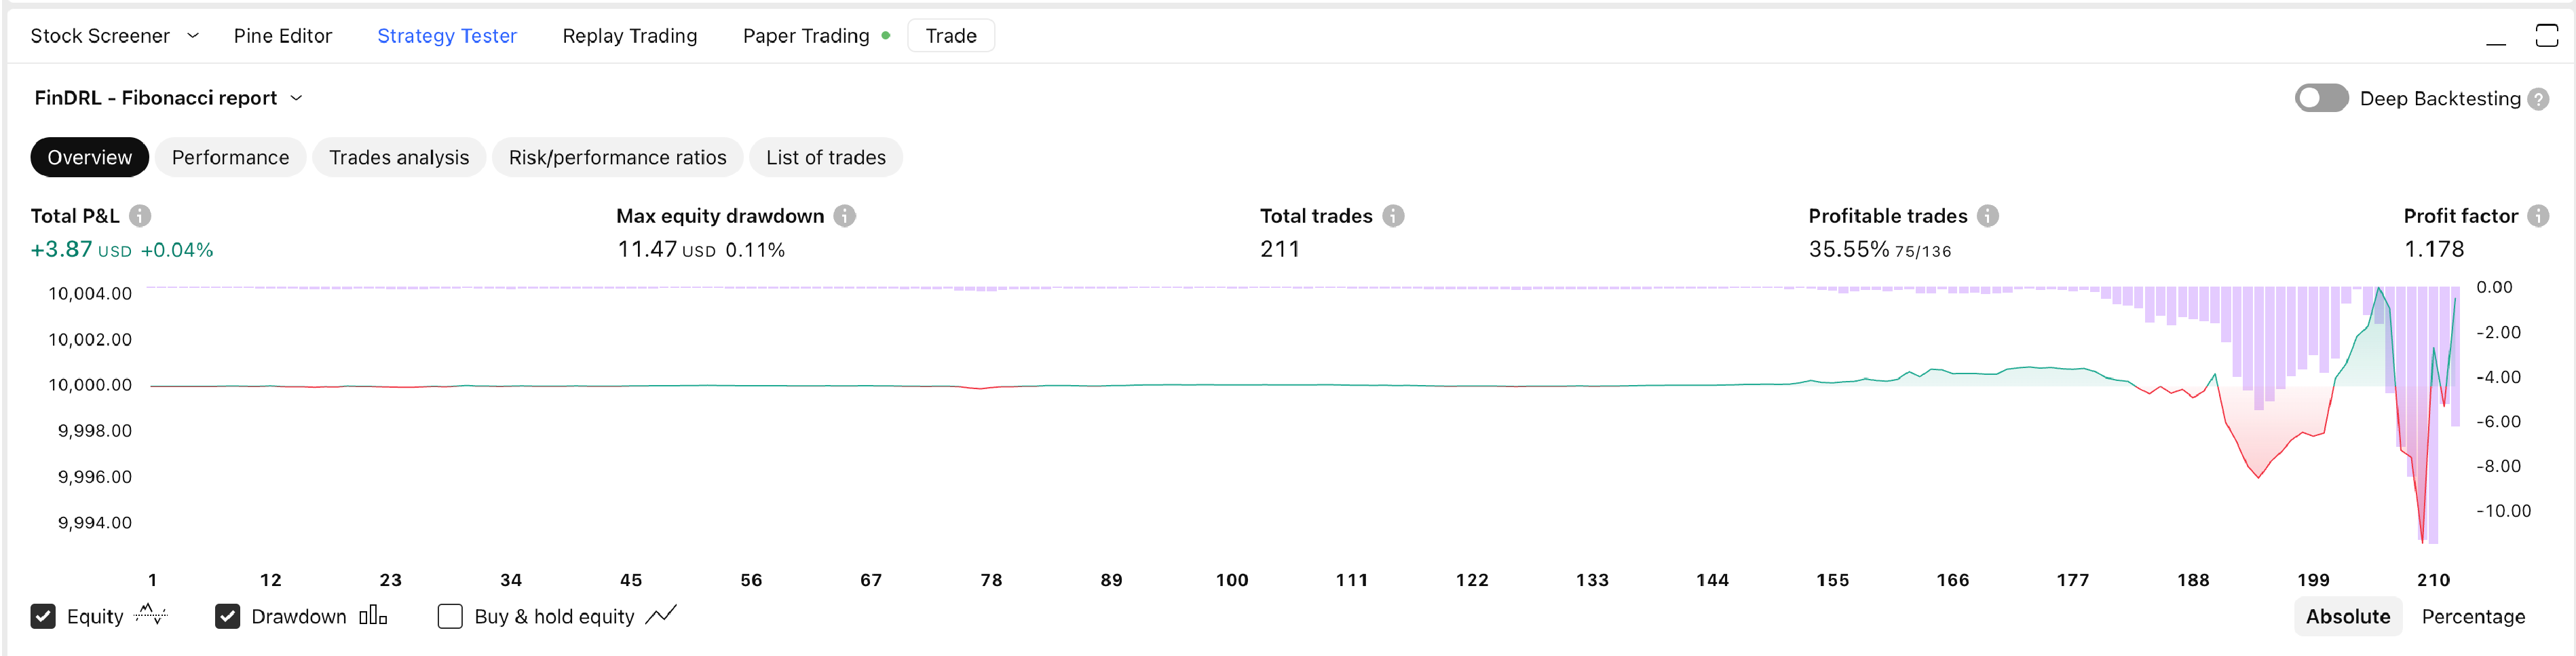
\includegraphics[width=.85\textwidth, height=3.6cm]{14-FinDRL-Fibonacci}
        \caption{Fibonacci Strategy Performance}
        \label{fig:Fibonacci performance}
    \end{figure}
    
    \item \textbf{FinDRL - Price Action}: Enters on bullish candles (close > open) when \%K crosses \%D. Backtesting from July 1, 2024, to February 26, 2025, yielded +15.05 USD (+0.15\%), 1,069 trades, 36.11\% win rate, 44.76 USD drawdown, and a profit factor of 1.141.

    \begin{figure}[htbp]
        \centering
        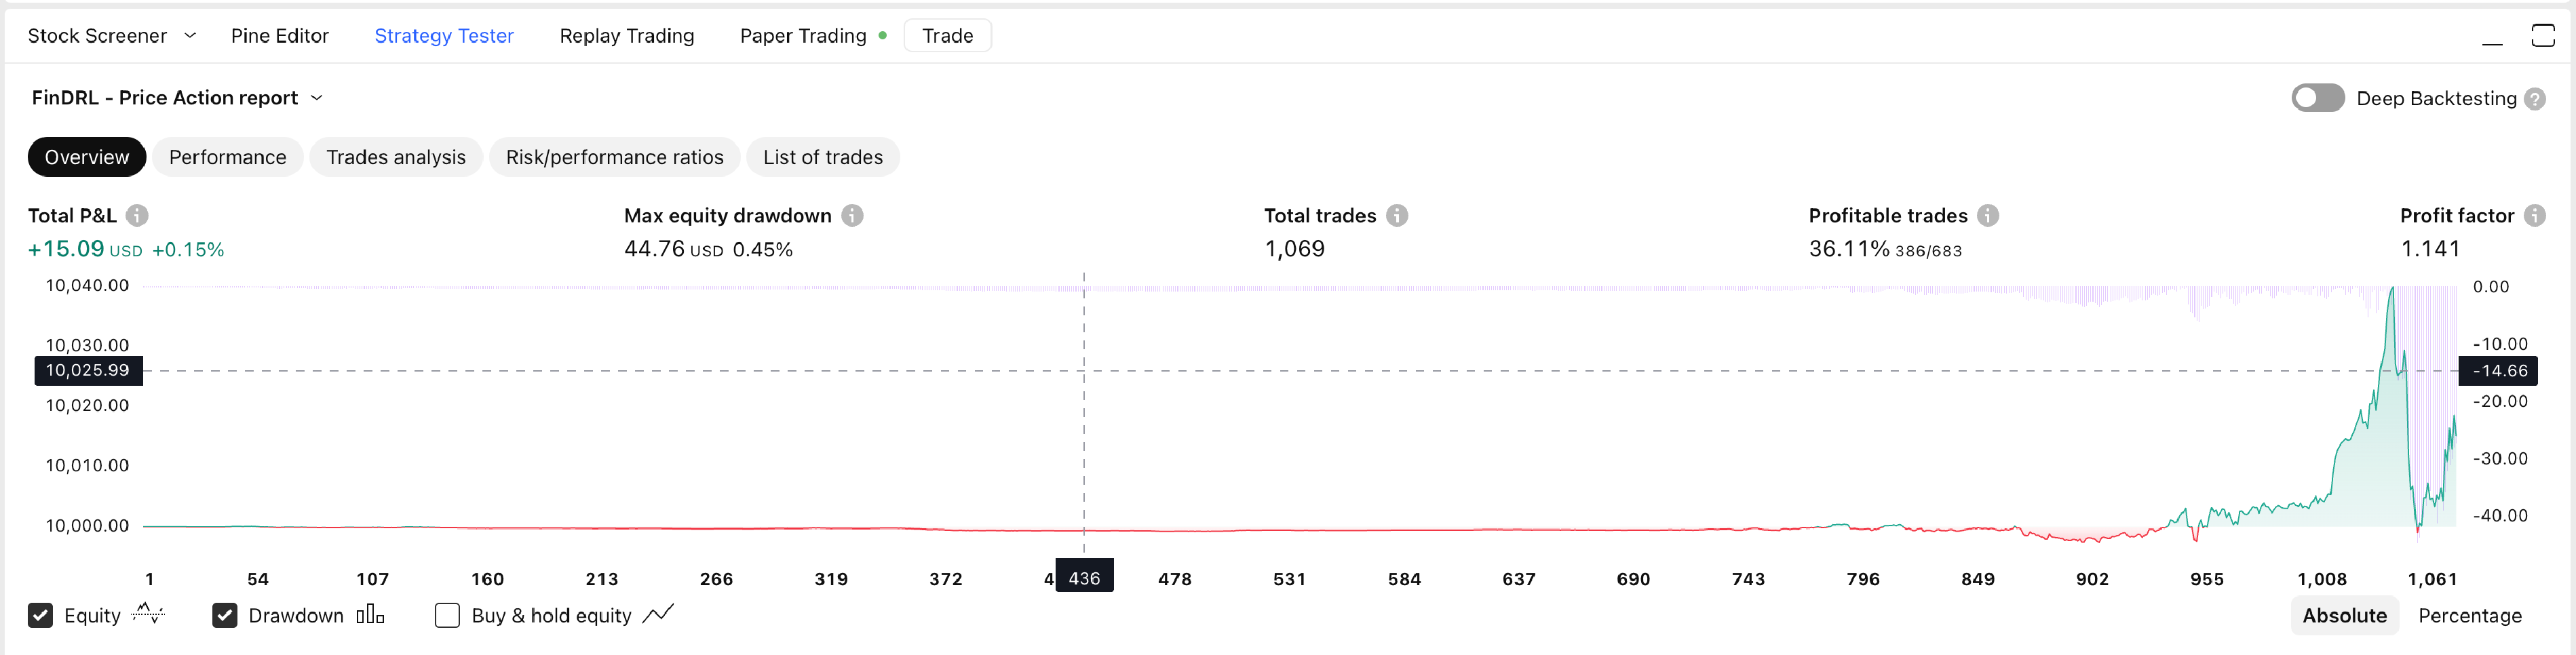
\includegraphics[width=.85\textwidth, height=3.6cm]{15-FinDRL-Price-Action}
        \caption{Price Action Strategy Performance}
        \label{fig:Price Action performance}
    \end{figure}
    
\end{itemize}
Mean-reversion strategies thrive in ranging markets, with FinDRL - Williams \%R and FinDRL - Stochastic RSI leading in profit factor, though FinDRL - RSI failed to trigger trades.

\subsection{Volume-Based Strategies}
\begin{itemize}
    \item \textbf{FinDRL - VWMA}: Enters when the price exceeds a 20-period Volume-Weighted Moving Average (VWMA), with \%K > \%D. The VWMA is \(\frac{\sum (\text{close} \times \text{volume})}{20} / \frac{\sum \text{volume}}{20}\). Backtesting from September 1, 2024, to February 26, 2025, resulted in +35.08 USD (+0.35\%), 912 trades, 35.09\% win rate, 34.98 USD drawdown, and a profit factor of 1.306.

    \begin{figure}[htbp]
        \centering
        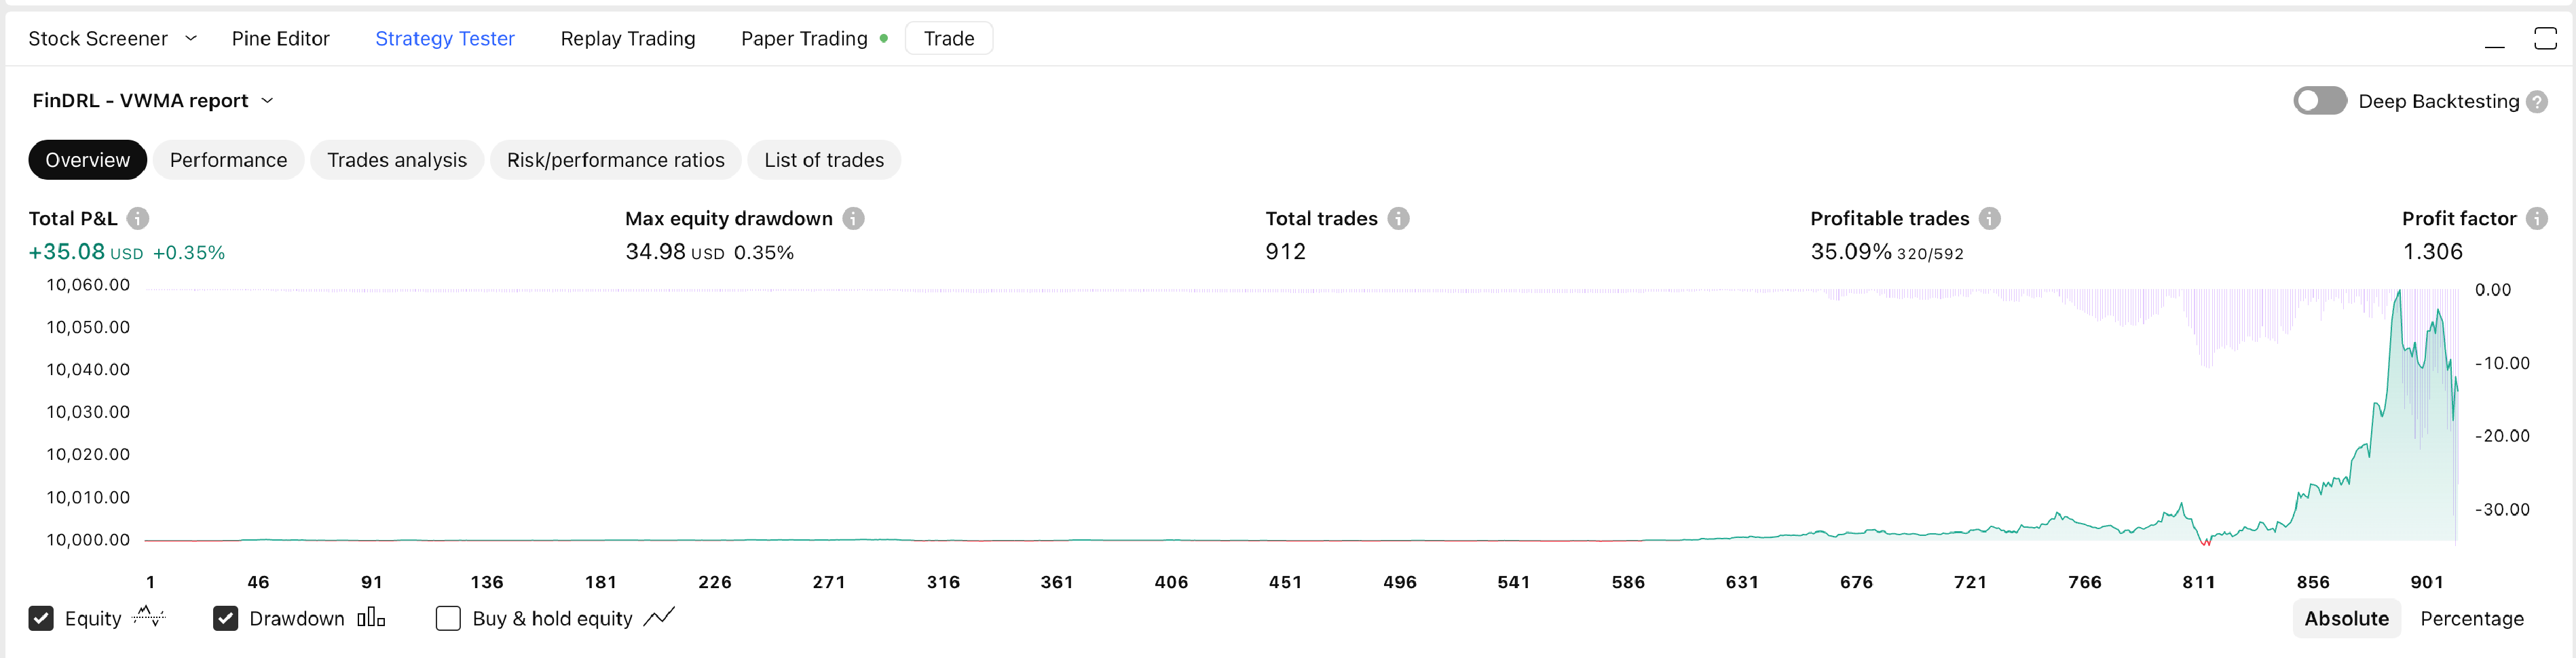
\includegraphics[width=.85\textwidth, height=3.6cm]{10-FinDRL-VWMA}
        \caption{VWMA Strategy Performance}
        \label{fig:VWMA performance}
    \end{figure}
    
    \item \textbf{FinDRL - CMF}: Enters when Chaikin Money Flow (CMF) > 0, with \%K > \%D. The CMF is \(\frac{\sum (\text{multiplier} \times \text{volume})}{20} / \frac{\sum \text{volume}}{20}\), where multiplier = \(\frac{((\text{close} - \text{low}) - (\text{high} - \text{close}))}{(\text{high} - \text{low})}\). Performance from July 1, 2024, to February 26, 2025, yielded +25.28 USD (+0.25\%), 852 trades, 34.86\% win rate, 48.04 USD drawdown, and a profit factor of 1.18.

    \begin{figure}[htbp]
        \centering
        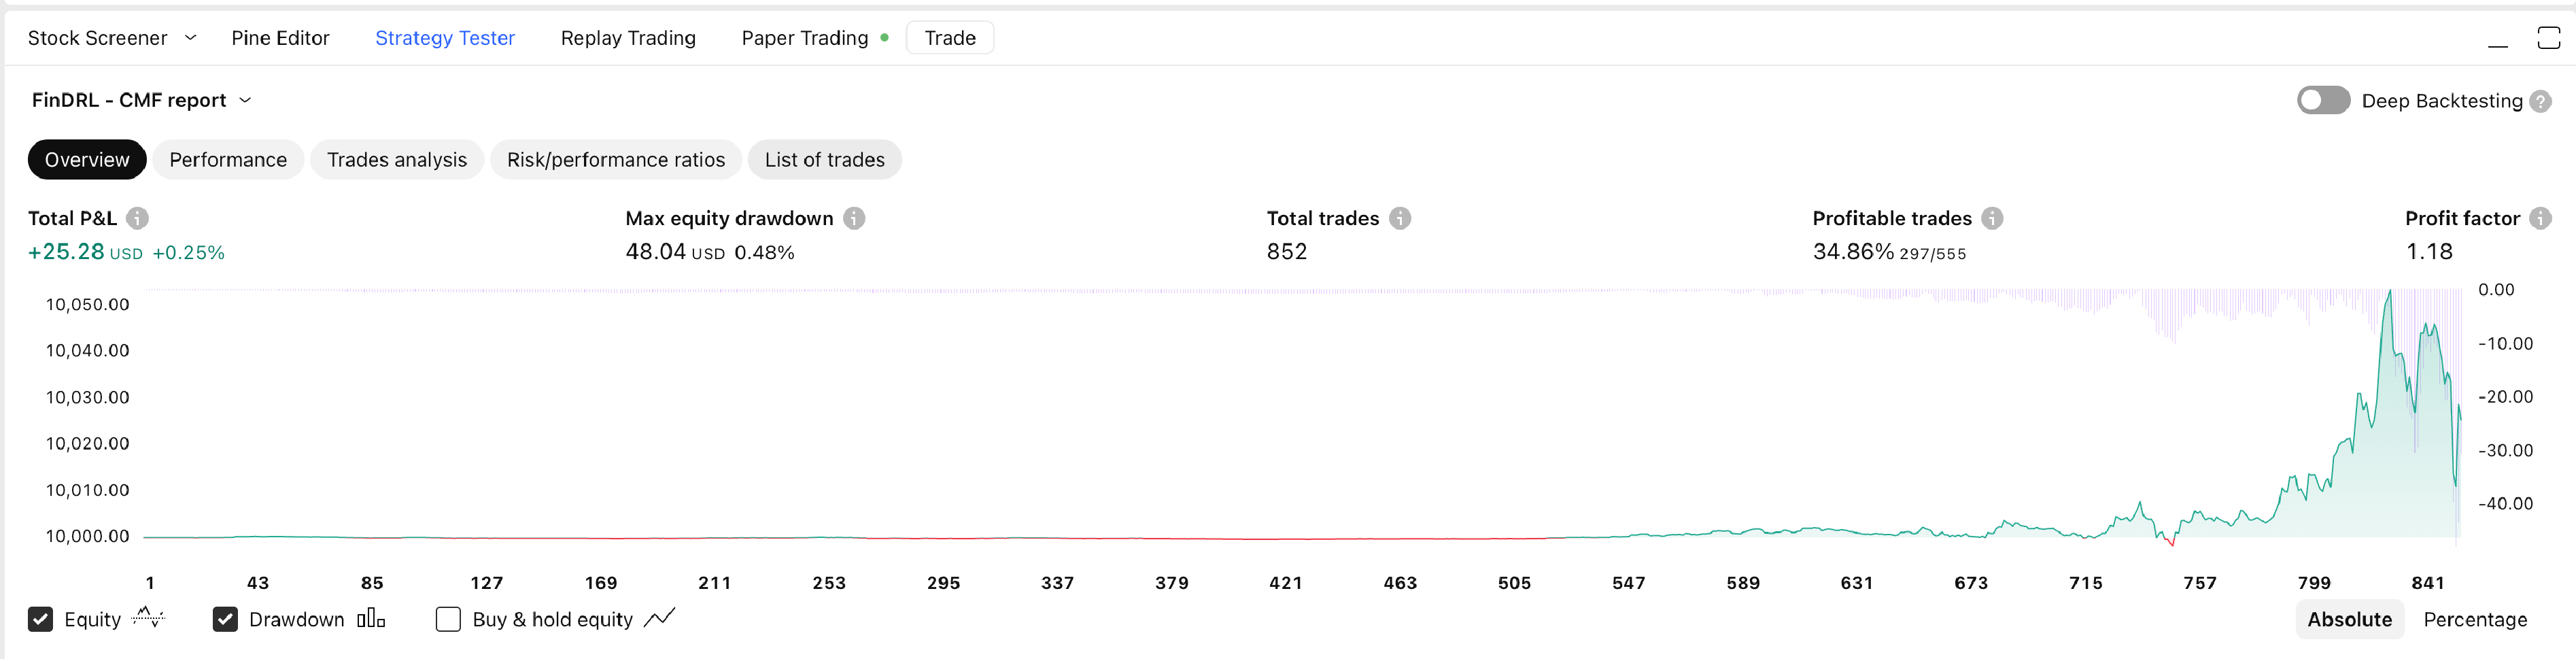
\includegraphics[width=.85\textwidth, height=3.6cm]{19-FinDRL-CMF}
        \caption{CMF Strategy Performance}
        \label{fig:CMF performance}
    \end{figure}
    
    \item \textbf{FinDRL - OBV}: Enters when On-Balance Volume (OBV) rises, with \%K crossing \%D. The OBV is \(\text{OBV}[1] + (\text{close} > \text{close}[1] ? \text{volume} : \text{close} < \text{close}[1] ? -\text{volume} : 0)\). Backtesting from October 1, 2008, to February 26, 2025, showed +21.46 USD (+0.21\%), 1,171 trades, 35.53\% win rate, 46.98 USD drawdown, and a profit factor of 1.187.

    \begin{figure}[htbp]
        \centering
        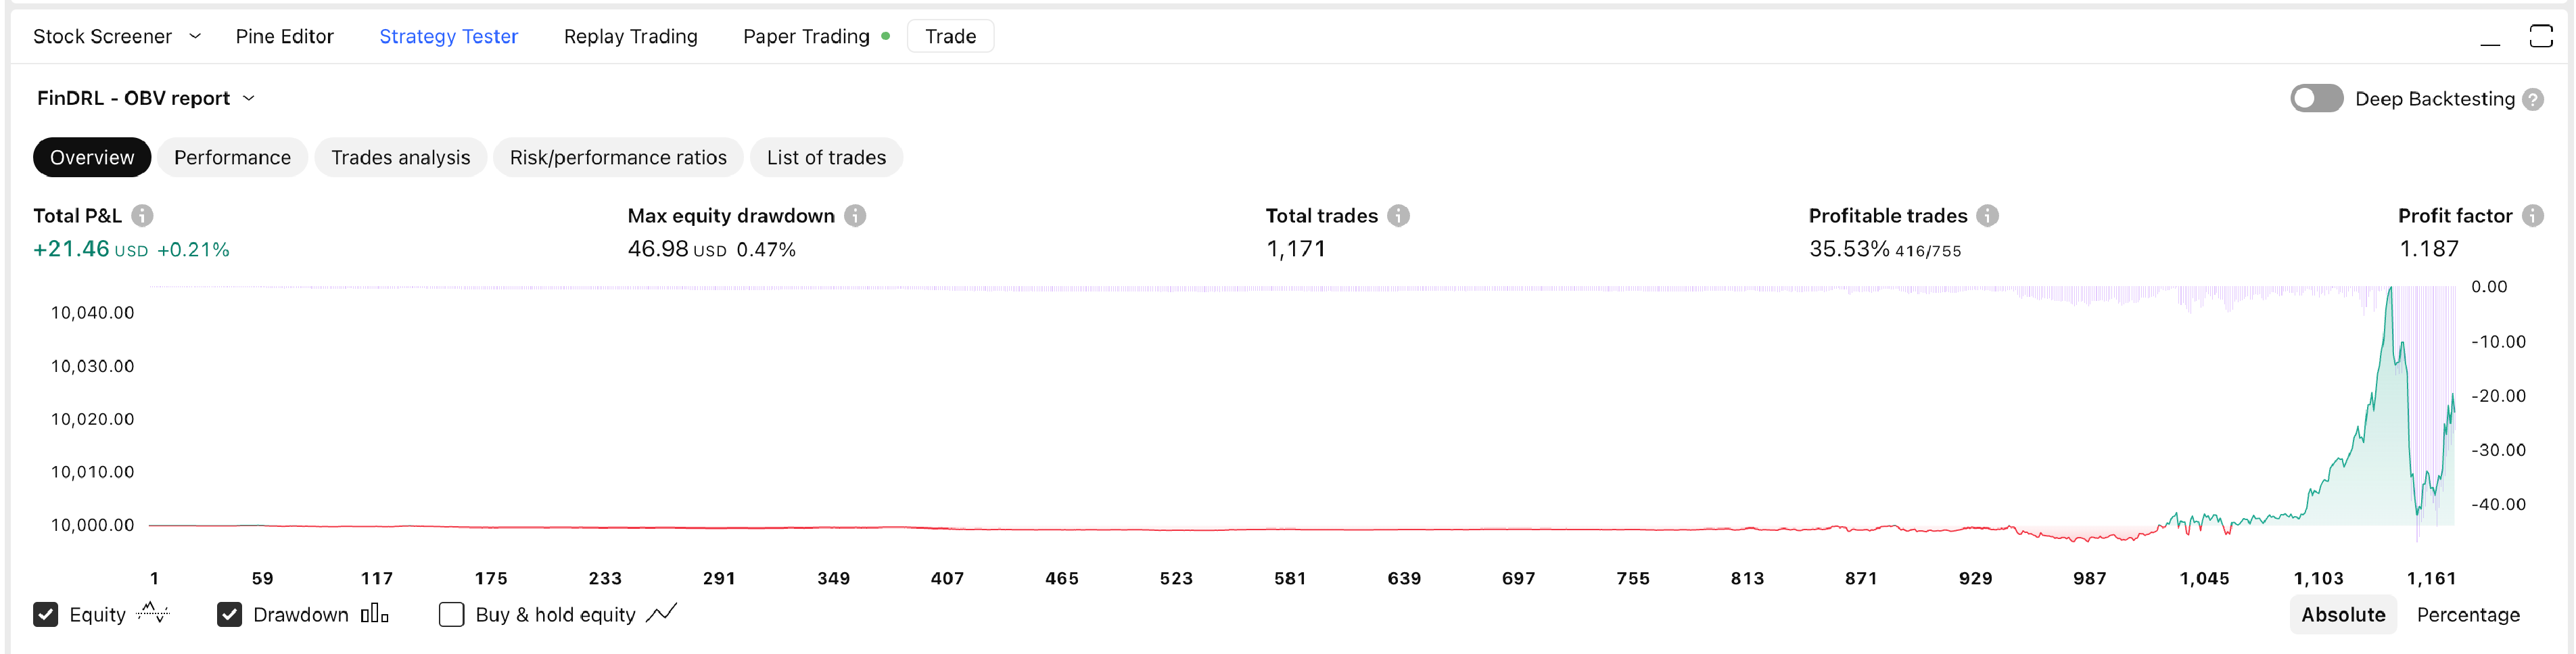
\includegraphics[width=.85\textwidth, height=3.6cm]{20-FinDRL-OBV}
        \caption{OBV Strategy Performance}
        \label{fig:OBV performance}
    \end{figure}
    
\end{itemize}
Volume-based strategies perform strongly in liquid, bullish markets, with FinDRL - VWMA achieving the highest profitability.

\section{Results and Discussion}
The 20 "FinDRL - *" signals from backtesting on 1D NVDA (NASDAQ) 2007-2025 produced mixed results. For instance, Momentum (net profit +38.62 USD; profit factor 1.257) and MACD (+27.69 USD; profit factor 1.287) are both trend-following and possess high win rates in extended uptrending environments. In addition, Williams \%R (+10.95 USD; profit factor 1.972) and Stochastic RSI (+13.60 USD; profit factor 1.669) are mean reversion strategies that produced the most profitability in non-trending or range-bound environments, where Williams \%R and Stochastic RSI could use their characteristics to leverage reversion to the mean with a high degree of efficiency. Volume seemingly was also an okay signal as well since VWMA (+35.08 USD; profit factor 1.306) and CMF (+25.28 USD; profit factor 1.18) had relatively better results, but Volume Spike (+7.69 USD; profit factor 2.469) had fewer trades (98) but a volume spike in profit factor.
The results from the breakout strategies were similarly ambiguous. Keltner Channel (+7.19 USD, profit factor 1.165) and Volume Spike hit take profit while Bollinger Bands (-0.78 USD, profit factor 0.975) and Parabolic SAR (-9.89 USD, profit factor 0.965) did not; but the latter two experienced similar patterns like prior which did not succeed in sideways/choppy volatility approaches. In addition, Donchian Channel, ATR, and RSI had no trade as well, which could indicate backtesting entry errors, adjustments not hitting parameters, or market conditions that did not hit thresholds to trigger signals either.
The implied notion that the 1D NVDA data was used throughout means that the simulations are effective no matter what the market. On the other hand, this is a downside because it only trades NVDA and the second strategy generated no trades. Maybe it needs further adjustment. If this project were to continue, further experimentation with different securities, different time frames, or even.

\begin{table}[h]
\caption{Summary of FinDRL Strategies}
\label{tab:result_strategies}
\tiny
\begin{tabular}{|l|c|c|c|c|c|c|c|}
\toprule
Strategy Name & Type & Net Profit (USD) & Win Rate (\%) & Max Drawdown (USD) & Trades & Profit Factor & Timeframe \& Asset (1D, NVDA)\\
\midrule
FinDRL - Gaussian Channel & Breakout        & +2.29           & 38.98        & 10.19              & 236    & 1.105         & Jan 01, 2023 - Nov 14, 2025 \\
FinDRL - MA Crossover     & Trend-Following & +25.22          & 38.09        & 30.48              & 995    & 1.246         & Jan 26, 2023 - Nov 17, 2025 \\
FinDRL - Bollinger Bands  & Breakout        & -0.78           & 35.06        & 13.16              & 251    & 0.975         & Jul 01, 2024 - Feb 26, 2025\\
FinDRL - Parabolic SAR    & Trend-Following & -9.89           & 39.24        & 26.64              & 869    & 0.965         & Aug 01, 2024 - Feb 26, 2025 \\
FinDRL - MACD             & Trend-Following & +27.69          & 37.60        & 24.83              & 960    & 1.287         & Aug 01, 2024 - Feb 26, 2025\\
FinDRL - Stochastic RSI   & Mean-Reversion  & +13.60          & 33.80        & 9.32               & 284    & 1.669         & Sep 15, 2009 - Feb 26, 2025\\
FinDRL - ADX              & Trend-Following & +32.74          & 33.71        & 50.43              & 887    & 1.253         & Aug 01, 2024 - Feb 26, 2025\\
FinDRL - VWMA             & Volume-Based    & +35.08          & 35.09        & 34.98              & 912    & 1.306         & Sep 01, 2024 - Feb 26, 2025\\
FinDRL - Donchian Channel & Breakout        & 0.00            & 0.00         & 0.00               & 0      & NA            & Sep 01, 2024 - Feb 26, 2025\\
FinDRL - SuperTrend       & Trend-Following & +5.02           & 36.09        & 15.78              & 266    & 1.202         & Jul 01, 2024 - Feb 26, 2025\\
FinDRL - Fibonacci        & Mean-Reversion  & +3.67           & 35.55        & 11.47              & 211    & 1.178         & Aug 26, 2024 - Feb 26, 2025\\
FinDRL - Price Action     & Mean-Reversion  & +15.05          & 36.11        & 44.76              & 1,069  & 1.141         & Jul 01, 2024 - Feb 26, 2025\\
FinDRL - Volume Spike     & Breakout        & +7.69           & 34.69        & 6.46               & 98     & 2.469         & Aug 15, 2024 - Feb 26, 2025\\
FinDRL - Momentum         & Trend-Following & +38.62          & 36.81        & 36.29              & 1,065  & 1.257         & Aug 01, 2024 - Feb 26, 2025\\
FinDRL - Williams \%R     & Mean-Reversion  & +10.95          & 29.89        & 7.10               & 184    & 1.972         & Jul 01, 2007 - Feb 26, 2025\\
FinDRL - CMF              & Volume-Based    & +25.28          & 34.86        & 48.04              & 852    & 1.18          & Jul 01, 2024 - Feb 26, 2025\\
FinDRL - OBV              & Volume-Based    & +21.46          & 35.53        & 46.98              & 1,171  & 1.187         & Oct 01, 2008 - Feb 26, 2025\\
FinDRL - Ichimoku Cloud   & Trend-Following & +20.03          & 31.82        & 69.96              & 330    & 1.218         & Jul 01, 2024 - Feb 26, 2025\\
FinDRL - ATR              & Breakout        & 0.00            & 0.00         & 0.00               & 0      & NA            & Sep 01, 2025 - Feb 26, 2025 \\
\bottomrule
\end{tabular}
\end{table}

\section{Conclusion and Future Work}
This chapter establishes a unified framework for designing and evaluating 20 “FinDRL - *” PineScript trading strategies, rigorously backtested on 1D NVDA (NASDAQ) from 2007 to 2025. The strategies provide a diverse toolkit for algorithmic trading, with Momentum and VWMA leading in profitability, and Williams \%R and Volume Spike excelling in risk-adjusted returns. However, the zero-trade results for Donchian Channel, ATR, and RSI highlight areas requiring refinement, potentially through parameter adjustment or market condition analysis.

Future work within this thesis will focus on validating these strategies through live trading, optimizing parameters for underperforming designs, and extending testing to multiple assets and timeframes to improve generalizability. Additionally, integrating machine learning techniques or adaptive algorithms could enhance the strategies’ adaptability to dynamic market conditions beyond historical data, contributing to the broader objectives of the dissertation.
